\documentclass[12pt,a4paper]{article}

% Packages
\usepackage[utf8]{inputenc}
\usepackage[T1]{fontenc}
\usepackage{lmodern}
\usepackage[margin=2.5cm]{geometry}
\usepackage{hyperref}
\usepackage{graphicx}
\usepackage{listings}
\usepackage{xcolor}
\usepackage{booktabs}
\usepackage{longtable}
\usepackage{array}
\usepackage{enumitem}
\usepackage{titlesec}
\usepackage{fancyhdr}
\usepackage{amsmath}
\usepackage{amssymb}
\usepackage{microtype}
\usepackage{parskip}
\usepackage{tikz}
\usepackage{float}
\usetikzlibrary{arrows.meta,positioning,backgrounds,fit}

% Hyperref setup
\hypersetup{
	colorlinks=true,
	linkcolor=blue!70!black,
	urlcolor=blue!70!black,
	citecolor=green!50!black,
	pdftitle={CyberShip Software Suite -- Architecture, Operation, and Configuration},
	pdfauthor={CyberShip Software Suite},
}

% Listings style
\definecolor{codebg}{HTML}{F5F5F5}
\definecolor{codeframe}{HTML}{CCCCCC}
\definecolor{keyword}{HTML}{0000AA}
\definecolor{comment}{HTML}{006600}
\definecolor{string}{HTML}{AA0000}

\lstdefinestyle{bash}{
	backgroundcolor=\color{codebg},
	frame=single,
	rulecolor=\color{codeframe},
	basicstyle=\ttfamily\small,
	keywordstyle=\color{keyword}\bfseries,
	commentstyle=\color{comment},
	stringstyle=\color{string},
	breaklines=true,
	breakatwhitespace=false,
	columns=fullflexible,
	postbreak=\mbox{\textcolor{gray}{$\hookrightarrow$}\space},
	showstringspaces=false,
	tabsize=2,
}

\lstdefinestyle{yaml}{
	backgroundcolor=\color{codebg},
	frame=single,
	rulecolor=\color{codeframe},
	basicstyle=\ttfamily\small,
	commentstyle=\color{comment},
	stringstyle=\color{string},
	breaklines=true,
	breakatwhitespace=false,
	columns=fullflexible,
	postbreak=\mbox{\textcolor{gray}{$\hookrightarrow$}\space},
	showstringspaces=false,
	tabsize=2,
}

% Header/Footer
\pagestyle{fancy}
\fancyhf{}
\fancyhead[L]{\small CyberShip Software Suite}
\fancyhead[R]{\small Architecture \& Operations Manual}
\fancyfoot[C]{\thepage}
\renewcommand{\headrulewidth}{0.4pt}

% Title
\title{
	\vspace{-1cm}
	\textbf{CyberShip Software Suite}\\[0.5em]
	\large Architecture, Operation, and Configuration Manual
}
\author{Marine Cybernetics Laboratory (MCLab)\\NTNU}
\date{June 2026}

\begin{document}
	
	\maketitle
	\thispagestyle{fancy}
	
	\tableofcontents
	\newpage
	
	% ============================================================
	\section{Introduction}
	\label{sec:intro}
	% ============================================================
	
	The \textbf{CyberShip Software Suite} is a collection of ROS~2 packages developed at the Marine
	Cybernetics Laboratory (MCLab) at NTNU. Together they provide a complete software stack for
	simulating, visualizing, and controlling autonomous maritime vessels. The suite covers everything
	from digital-twin URDF models and real-time sensor integration (IMU, motion capture) to advanced
	control algorithms (dynamic positioning, thrust allocation).
	
	The suite is published on GitHub at
	\url{https://github.com/NTNU-MCS/cybership_software_suite} and archived on Zenodo
	(DOI: \texttt{10.5281/zenodo.17233653}).
	
	\subsection{Supported Vessels}
	
	Three vessel models are currently supported:
	
	\begin{description}[leftmargin=3cm, style=nextline]
		\item[Voyager] Compact vessel used for general control experiments.
		\item[Enterprise] Medium-size vessel; simulation supported.
		\item[Drillship] Large vessel with dedicated launch configuration.
	\end{description}
	
	% ============================================================
	\section{Package Overview}
	\label{sec:packages}
	% ============================================================
	
	The repository is organized as a collection of focused ROS~2 packages. Table~\ref{tab:packages}
	summarizes each package and its primary responsibility.
	
	\begin{longtable}{@{}p{5.2cm}p{8.8cm}@{}}
		\toprule
		\textbf{Package}                & \textbf{Description}                                                                                           \\
		\midrule
		\endhead
		\texttt{cybership\_bringup}     & Launch files that orchestrate the complete startup of a vessel (hardware drivers, localization, sensor nodes). \\
		\addlinespace
		\texttt{cybership\_simulator}   & Lightweight Python simulation scripts based on simplified vessel physics.                                      \\
		\addlinespace
		\texttt{cybership\_viz}         & RViz configurations and launch files for real-time vessel visualization.                                       \\
		\addlinespace
		\texttt{cybership\_description} & URDF models, meshes, and coordinate-frame definitions for each vessel.                                         \\
		\addlinespace
		\texttt{cybership\_config}      & Centralized YAML configuration files shared across the suite.                                                  \\
		\addlinespace
		\texttt{cybership\_interfaces}  & Custom ROS~2 message and service definitions for maritime operations.                                          \\
		\addlinespace
		\texttt{cybership\_controller}  & Base package for vessel controllers.                                                                           \\
		\addlinespace
		\texttt{cybership\_dp}          & Dynamic positioning controllers (force and velocity).                                                          \\
		\addlinespace
		\texttt{cybership\_thrusters}   & Low-level thruster drivers supporting VSP, fixed, and azimuth types.                                           \\
		\addlinespace
		\texttt{cybership\_mocap}       & ROS~2 bridge to the Qualisys motion capture system.                                                            \\
		\addlinespace
		\texttt{cybership\_utilities}   & Shared helper functions, launch argument definitions, and GUI tools.                                           \\
		\addlinespace
		\texttt{cybership\_external}    & Third-party submodule dependencies (IMU driver, Dynamixel, PCA9685, etc.).                                     \\
		\addlinespace
		\texttt{cybership\_tests}       & Integration and unit tests for the suite.                                                                      \\
		\bottomrule
		\caption{CyberShip Software Suite packages.}
		\label{tab:packages}
	\end{longtable}
	
	% ============================================================
	\section{System Architecture}
	\label{sec:architecture}
	% ============================================================
	
	\subsection{High-Level Architecture}
	
	The system follows a layered ROS~2 architecture. Data flows from physical sensors upward through
	localization and state estimation to high-level control, then back down through thrust allocation to
	the actuators.
	
	\begin{enumerate}
		\item \textbf{Sensor layer} -- IMU (BNO055), motion capture (Qualisys).
		\item \textbf{Localization layer} -- \texttt{robot\_localization} EKF fuses sensor data into
		a consistent odometry estimate.
		\item \textbf{Control layer} -- Dynamic positioning controllers compute force and torque demands.
		\item \textbf{Actuation layer} -- The thruster package converts force demands to actuator
		signals (PWM, RPM, servo angle).
		\item \textbf{Hardware layer} -- PCA9685 PWM board, Dynamixel azimuth servos.
	\end{enumerate}
	
	\subsection{Distributed ROS~2 Network}
	
	The system runs as a distributed ROS~2 network across multiple machines. The
	\textbf{cybership-master} Raspberry Pi (\texttt{192.168.1.102}) acts as the
	\textbf{Fast~DDS discovery server} for all participants. Vessels run their own bringup as
	systemd user services and connect back to the discovery server automatically.
	
	\begin{center}
		\begin{tabular}{ll}
			\toprule
			\textbf{Host}                      & \textbf{Role / Address}                             \\
			\midrule
			\texttt{cybership-master.local}    & Discovery server, UI host -- \texttt{192.168.1.102} \\
			\texttt{cybership-voyager.local}   & Vessel node                                         \\
			\texttt{cybership-drillship.local} & Vessel node                                         \\
			\texttt{192.168.1.10}              & Qualisys motion capture system (read-only)          \\
			\bottomrule
		\end{tabular}
	\end{center}
	
	\subsection{Coordinate Frames}
	
	The vessels use two main coordinate frames defined in \texttt{cybership\_description}:
	
	\begin{description}[leftmargin=3.5cm]
		\item[\texttt{base\_link}] East-North-Up (ENU) frame. All sensors are defined here.
		\item[\texttt{base\_link\_ned}] North-East-Down (NED) frame. Used for navigation and control.
	\end{description}
	
	The NED frame is obtained by a static transform applied to the ENU frame.
	
	\subsection{Network Topology}
	
	Figure~\ref{fig:topology} shows the physical network layout of the CyberShip lab. All machines
	communicate over a shared \texttt{192.168.1.1/24} Wi-Fi LAN. The \textbf{cybership-master}
	Raspberry~Pi acts as the central hub: it runs the Fast~DDS discovery server (port~11811),
	serves the web UI (port~8001), and hosts any lab-side ROS~2 nodes. Vessel Raspberry~Pis register
	with the discovery server automatically at boot. Student workstations join by exporting
	\texttt{ROS\_DISCOVERY\_SERVER} in their shell environment.
	
	\begin{figure}[htbp]
		\centering
		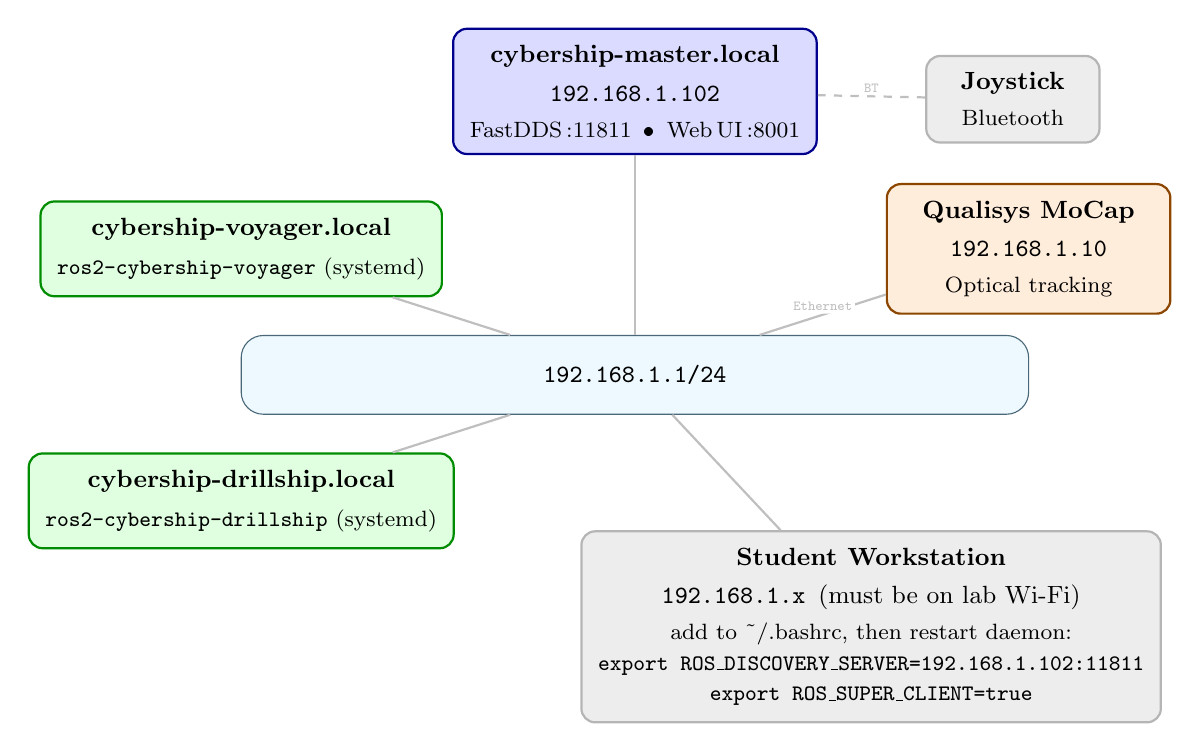
\begin{tikzpicture}[
			mach/.style={draw, rounded corners=5pt, minimum width=3.6cm,
				align=center, font=\small, thick, inner sep=6pt},
			masternd/.style={mach, fill=blue!14,   draw=blue!55!black},
			vesselnd/.style={mach, fill=green!12,  draw=green!55!black},
			mocapnd/.style ={mach, fill=orange!14, draw=orange!55!black},
			clientnd/.style={mach, minimum width=5.2cm, fill=gray!14, draw=gray!58},
			joynd/.style   ={mach, minimum width=2.2cm, fill=gray!14, draw=gray!58},
			netbus/.style  ={draw, fill=cyan!7, draw=cyan!40!black, rounded corners=8pt,
				minimum width=10cm, minimum height=1.0cm,
				align=center, font=\small\bfseries},
			wlink/.style={thick, gray!50},
			clink/.style={thick, gray!50},
			btlink/.style={thick, gray!50, dashed},
			ann/.style={font=\tiny\ttfamily, fill=white, inner sep=1pt, rounded corners=1pt},
			]
			
			%% ── Network backbone ─────────────────────────────────────────────────────────
			\node[netbus] (net) at (0, 0)
			{\texttt{192.168.1.1/24}};
			
			%% ── cybership-master ─────────────────────────────────────────────────────────
			\node[masternd] (master) at (0, 3.6)
			{\textbf{cybership-master.local}\\[3pt]
				\texttt{192.168.1.102}\\[2pt]
				{\footnotesize FastDDS\,:11811\enspace\textbullet\enspace Web\,UI\,:8001}};
			
			%% ── Vessel Raspberry Pis ─────────────────────────────────────────────────────
			\node[vesselnd] (voyager) at (-5.0, 1.6)
			{\textbf{cybership-voyager.local}\\[3pt]
				{\footnotesize \texttt{ros2-cybership-voyager} (systemd)}};
			
			\node[vesselnd] (drillship) at (-5.0, -1.6)
			{\textbf{cybership-drillship.local}\\[3pt]
				{\footnotesize \texttt{ros2-cybership-drillship} (systemd)}};
			
			%% ── Qualisys motion capture ──────────────────────────────────────────────────
			\node[mocapnd] (qualisys) at (5.0, 1.6)
			{\textbf{Qualisys MoCap}\\[3pt]
				\texttt{192.168.1.10}\\[2pt]
				{\footnotesize Optical tracking}};
			
			%% ── Student / operator workstation ──────────────────────────────────────────
			\node[clientnd] (laptop) at (3, -3.2)
			{\textbf{Student Workstation}\\[3pt]
				\texttt{192.168.1.x}\enspace(must be on lab Wi-Fi)\\[2pt]
				{\footnotesize add to \textasciitilde/.bashrc, then restart daemon:}\\
				{\footnotesize \texttt{export ROS\_DISCOVERY\_SERVER=192.168.1.102:11811}}\\
				{\footnotesize \texttt{export ROS\_SUPER\_CLIENT=true}}};
			
			%% ── Bluetooth joystick (connects to master) ──────────────────────────────────
			\node[joynd] (joy) at (4.8, 3.5)
			{\textbf{Joystick}\\[2pt]
				{\footnotesize Bluetooth}};
			
			%% ── Wi-Fi links ──────────────────────────────────────────────────────────────
			\draw[wlink] (master)   -- (net);
			\draw[wlink] (voyager)  -- (net);
			\draw[wlink] (drillship)-- (net);
			\draw[wlink] (laptop)   -- (net);
			
			%% ── Ethernet cable: master ↔ Qualisys ───────────────────────────────────────
			\draw[clink] (qualisys) -- node[ann, above]{\tiny Ethernet} (net);
			
			%% ── Bluetooth link ───────────────────────────────────────────────────────────
			\draw[btlink] (joy) -- node[ann, above]{\tiny BT} (master);
			
			
			
		\end{tikzpicture}
		\caption{Physical network topology of the CyberShip lab. Vessels and workstations
			communicate over the \texttt{192.168.1.1/24} Wi-Fi network.
			\textbf{cybership-master} is connected to the Qualisys system via a dedicated Ethernet
			cable and acts as the Fast~DDS discovery server for all ROS~2 participants.
			The Bluetooth joystick pairs with the master and its events are forwarded as ROS~2
			topics across the network.}
		\label{fig:topology}
	\end{figure}
	
	% ============================================================
	\section{Installation}
	\label{sec:installation}
	% ============================================================
	
	Installation instructions are maintained in the repository \texttt{README.md} and kept
	up to date with each release. Refer to:
	
	\begin{center}
		\url{https://github.com/NTNU-MCS/cybership_software_suite#installation}
	\end{center}
	
	% ============================================================
	\section{Network and Discovery Server Configuration}
	\label{sec:network}
	% ============================================================
	
	\noindent\fbox{\parbox{\dimexpr\linewidth-2\fboxsep-2\fboxrule\relax}{%
			\textbf{Note:} The IP addresses listed throughout this document reflect the current lab
			configuration and are subject to change. If an address does not respond, verify the
			current assignment with the lab supervisor before attempting further troubleshooting.
	}}
	
	\bigskip
	
	The CyberShip lab uses a dedicated \texttt{192.168.1.1/24} subnet. All machines (vessels, lab
	computers, and the master node) must be on this subnet.
	
	\subsection{Connecting a Workstation}
	
	Add the following lines to \texttt{\textasciitilde/.bashrc} on any machine that needs to join the
	ROS~2 network:
	
	\begin{lstlisting}[style=bash]
		export ROS_DISCOVERY_SERVER="192.168.1.102:11811"
		export ROS_SUPER_CLIENT=true
	\end{lstlisting}
	
	After editing, restart the ROS~2 daemon:
	
	\begin{lstlisting}[style=bash]
		ros2 daemon stop ; ros2 daemon start
	\end{lstlisting}
	
	\subsection{Virtual Machine Setup}
	
	Students using a virtual machine must set their VM network adapter to \textbf{Bridged} mode and
	select the Wi-Fi adapter as the bridged interface. Verify the assigned IP is in the
	\texttt{192.168.1.1/24} range with \texttt{ip addr}.
	
	\subsection{SSH Access}
	
	\begin{lstlisting}[style=bash]
		ssh mclab@cybership-master.local
		ssh mclab@cybership-voyager.local
		ssh mclab@cybership-drillship.local
	\end{lstlisting}
	
	\textbf{Tip:} Always use \texttt{tmux} when working on \texttt{cybership-master} so sessions
	persist across disconnections.
	
	% ============================================================
	\section{Bringing Up a Vessel}
	\label{sec:bringup}
	% ============================================================
	
	\subsection{Automatic Startup}
	
	Each vessel automatically starts its bringup at boot via a \textbf{systemd user service} named
	\texttt{ros2-cybership-<vessel\_model>}. The service runs:
	
	\begin{lstlisting}[style=bash]
		ros2 launch cybership_bringup all.launch.xml
	\end{lstlisting}
	
	You do not normally need to SSH into the vessel; simply powering it on (connecting the battery)
	is sufficient.
	
	\subsection{Manual Bringup}
	
	To manually launch bringup for a vessel, use the corresponding launch file from
	\texttt{cybership\_bringup}:
	
	\begin{lstlisting}[style=bash]
		# Voyager
		ros2 launch cybership_bringup voyager.launch.py \
		vessel_name:=voyager vessel_model:=voyager
		
		# Enterprise
		ros2 launch cybership_bringup enterprise.launch.py
		
		# Drillship
		ros2 launch cybership_bringup drillship.launch.py
	\end{lstlisting}
	
	\subsection{Bringup Include Files}
	
	The bringup package composes several include launch files, each starting a specific subsystem:
	
	\begin{description}[leftmargin=5cm, style=nextline]
		\item[\texttt{azimuth\_controller.launch.py}]
		Starts the Dynamixel azimuth servo controller node.
		\item[\texttt{imu\_bno055.launch.py}]
		Starts the BNO055 IMU driver node.
		\item[\texttt{motion\_capture\_system\_connector.launch.py}]
		Connects to the Qualisys motion capture server and retrieves rigid-body poses.
		\item[\texttt{motion\_capture\_system\_transformer.launch.py}]
		Transforms raw mocap data into the vessel's coordinate frame.
		\item[\texttt{robot\_localization.launch.py}]
		Runs the \texttt{robot\_localization} EKF node to fuse IMU and mocap data.
		\item[\texttt{servo\_driver.launch.py}]
		Starts the servo driver node (PCA9685-based).
		\item[\texttt{thruster\_control.launch.py}]
		Starts the thruster controller nodes.
		\item[\texttt{urdf\_description.launch.py}]
		Publishes the URDF model via \texttt{robot\_state\_publisher}.
		\item[\texttt{localization.launch.py}]
		Top-level localization launch combining the above components.
	\end{description}
	
	% ============================================================
	\section{Localization}
	\label{sec:localization}
	% ============================================================
	
	Vessel localization fuses two complementary sensor streams:
	
	\begin{enumerate}
		\item \textbf{BNO055 IMU} -- Provides 9-DOF inertial measurements (accelerometer, gyroscope,
		magnetometer). Integrated via the \texttt{bno055} ROS~2 driver in
		\texttt{cybership\_external}.
		\item \textbf{Qualisys motion capture} -- Provides absolute 6-DOF pose measurements at
		\texttt{192.168.1.10} using the \texttt{mocap4ros2\_qualisys} driver and
		\texttt{cybership\_mocap} bridge.
	\end{enumerate}
	
	The fused estimate is produced by the \texttt{robot\_localization} Extended Kalman Filter (EKF)
	node. Convergence of the EKF can be monitored by inspecting the covariance matrix on the
	\texttt{/<vessel\_name>/measurement/odom} topic or by watching the vessel in RViz.
	
	\subsection{Motion Capture Node Details}
	
	The \texttt{cybership\_mocap} package subscribes to the \texttt{rigid\_bodies} topic
	(\texttt{mocap4r2\_msgs/msg/RigidBodies}) and republishes pose data as
	\texttt{geometry\_msgs/msg/PoseWithCovarianceStamped}. Key configuration parameters are shown
	in Table~\ref{tab:mocap_params}.
	
	\begin{table}[ht]
		\centering
		\begin{tabular}{llp{5cm}l}
			\toprule
			\textbf{Parameter}         & \textbf{Type} & \textbf{Description}        & \textbf{Default}              \\
			\midrule
			\texttt{world\_frame}      & string        & Global reference frame name & \texttt{mocap}                \\
			\texttt{base\_frame}       & string        & Robot base frame            & \texttt{cybership/base\_link} \\
			\texttt{rigid\_body\_name} & string        & Name in mocap system        & \texttt{cybership}            \\
			\texttt{topic\_name}       & string        & Output pose topic           & \texttt{cybership/pose}       \\
			\texttt{publish\_tf}       & bool          & Broadcast TF transform      & \texttt{true}                 \\
			\bottomrule
		\end{tabular}
		\caption{Motion capture node configuration parameters.}
		\label{tab:mocap_params}
	\end{table}
	
	\textbf{Important}: The order in which rigid bodies are registered in the Qualisys software
	determines their index. Ensure the order matches the vessel being launched.
	
	% ============================================================
	\section{Motion Capture System}
	\label{sec:mocap}
	% ============================================================
	
	\subsection{Startup Procedure}
	
	This section describes the standard startup procedure for most users of the Cybership vessels in the MC Lab. If your project requires a different setup or configuration, contact the laboratory engineers before proceeding.
	
	\subsubsection{Quick Startup Checklist}
	
	Begin with this short checklist if you already know the QTM workflow:
	
	\begin{enumerate}
		\item[$\square$] Open the \textit{Qualisys\_Default\_MCLab} project in QTM.
		\item[$\square$] Open a new measurement window.
		\item[$\square$] Verify that all cameras are connected and that the expected number of cameras is shown.
		\item[$\square$] Check that the vessel appears in 6DOF view with the correct rigid body definition, and that the vessels are in the correct order. 
		\item[$\square$] Confirm that the residual is sufficiently low before starting an experiment.
	\end{enumerate}
	
	\subsubsection{Qualisys Track Manager Startup}
	
	Use the computer labeled \textit{QTM Surface} (IP address: \texttt{192.168.1.10}).
	
	Open QTM (Qualisys Track Manager). When the \textit{Manage Projects} window appears, select \texttt{Qualisys\_Default\_MCLab}. Press \texttt{Ctrl + N} to open a new measurement window.
	
	Verify that the number of connected cameras displayed in the status bar matches the number of cameras currently in use (the default configuration uses seven cameras).
	
	In the toolbar on the left, select \textit{3D View}. This displays the laboratory coordinate system, which is defined as follows:
	
	\begin{itemize}
		\item The $x$-axis points toward the wavemaker.
		\item The $z$-axis points downward.
		\item The $y$-axis completes the right-handed coordinate system and points from the gangway toward the opposite side of the basin.
		\item The origin is located as close to the center of the basin as possible. At the time of writing, its exact position may vary between calibrations.
		\item The coordinate system orientation and origin location are established during calibration, which is normally performed by laboratory personnel. If your project requires the exact origin position or a different coordinate system orientation, contact the laboratory engineers before starting.
	\end{itemize}
	
	Press \texttt{Ctrl + D} to open the \textit{Data Info} window. By default, this window displays marker data and coordinates.
	
	Right-click anywhere in the window and select \textit{Display 6DOF Data}. The window will then display the position and orientation of all defined rigid bodies:
	
	\[
	x,\; y,\; z,\; \text{roll},\; \text{pitch},\; \text{yaw}
	\]
	
	The displayed data also includes the \textit{residual}\footnote{
		The rigid body residual is the average error, measured in millimeters, between the observed marker positions and the corresponding points in the rigid body definition.
		\url{https://docs.qualisys.com/qtm/content/qtm_user_interface/qtm_windows/6dof_data_information.htm?Highlight=residual}
	}.
	
	Note that QTM displays position coordinates ($x$, $y$, and $z$) in millimeters and orientation angles (roll, pitch, and yaw) in degrees.
	
	You may now place the vessel in the basin. If the vessel is tracked correctly in QTM and the residual is sufficiently low, the system is ready for use. Residuals may increase in regions with limited camera coverage or areas that were not fully included during calibration. The calibrated volume can be visualized by pressing \texttt{Alt + 7}.
	
	If the vessel is not detected correctly, or the residual remains high ($>1$ mm), continue to Section~\ref{sec:rigidbody}.
	
	\subsubsection{Rigid Body Setup and Verification}
	\label{sec:rigidbody}
	
	If the vessel has not already been defined, or if you are using a different vessel, the corresponding rigid body definitions must be loaded or created.
	
	Open the \textit{Project Options} window by clicking the gear icon in the upper-left toolbar. Navigate to \textit{Processing} $\rightarrow$ \textit{6DOF Tracking}.
	
	For the default MC Lab vessels, select \textit{Load Bodies} in the lower-right corner and load the file
	
	\begin{center}
		\texttt{MCLab\_default.xml}
	\end{center}
	
	which contains the predefined rigid body definitions.
	
	If the vessel has not previously been defined, or if you need to create a new rigid body definition, follow the procedure described below.
	
	% Add rigid body creation procedure here.
	
	Place the vessel in the basin. Only one vessel should be present during rigid body acquisition. Remove other vessels from the basin or cover their markers to prevent false detections. Keep the vessel in view of as many cameras as possible; clicking \textit{2D} on the left returns you to \textit{camera view}, which is useful here. The initial position ($x$, $y$, $z$) does not matter, but make sure that the vessel heading is aligned with the desired heading corresponding to $0^\circ$ yaw. If your experiment requires it, also make sure that the vessel is balanced, because QTM sets $(roll, pitch, yaw) = (0, 0, 0)$ when you acquire a rigid body. 
	
	Go to the \textit{6DOF Settings} window in \textit{Project Options} and press \textit{Acquire Body}. Verify that the body has been detected, then click \textit{Apply} and \textit{OK}. Close the measurement window by pressing the lower of the two crosses in the top right corner. Open a new measurement window and repeat the steps until you see the rigid body coordinates in 6DOF. 
	
	For first-time users it may seem that everything is in order. The rigid body defined by the markers and its coordinates in 6DOF should both be visible, but QTM uses the centroid of the marker constellation as the body frame origin, which does not correspond to the vessel geometric center. To correct this, all Cybership vessels should have a reference marker marked by a black line on the marker stem, with its position relative to the vessel geometric center and waterline written near it. The current values at the time of writing are listed below for Voyager (Table~\ref{tab:voyager_ref_marker}) and Drillship (Table~\ref{tab:drillship_ref_marker}).
	
	\begin{table}[h]
		\centering
		\caption{Voyager Reference Marker Coordinates}
		\label{tab:voyager_ref_marker}
		\begin{tabular}{l c}
			\hline
			Coordinate & Value [mm] \\
			\hline
			$x$ & 29 \\
			$y$ & 125 \\
			$z$ & -185 \\
			\hline
		\end{tabular}
	\end{table}
	
	\begin{table}[h]
		\centering
		\caption{Drillship Reference Marker Coordinates}
		\label{tab:drillship_ref_marker}
		\begin{tabular}{l c}
			\hline
			Coordinate & Value [mm] \\
			\hline
			$x$ & 158 \\
			$y$ & 187.5 \\
			$z$ & -225 \\
			\hline
		\end{tabular}
	\end{table}
	
	Find the marker in QTM corresponding to the reference marker on the vessel. Select the marker and note its label. The label will typically have the format \texttt{Body1-x}, although it may instead appear as \texttt{Voyager-y} or a similar name if the rigid body has previously been renamed. Return to \emph{6DOF Tracking} settings, select the rigid body, and click \emph{Translate}. Select the option: 
	
	\begin{center}
		\emph{So that point \textlangle LABEL\textrangle in the body has local coordinates(in mm):}
	\end{center}
	Enter the values for the vessel in question and press \emph{OK}, then press \emph{Apply} and verify that the body origin has moved to the correct location. 
	\subsubsection{Streaming Output Verification}
	
	After QTM is configured, confirm that the 6DOF data stream is visible to downstream ROS~2 nodes. Verify that pose updates are being published and that the vessel appears at the expected position in RViz or any other consumer of the mocap topic. Make sure that the rigid bodies are in the correct order expected by the ROS~2 mocap nodes, Voyager at the top and then Drillship.  If no data appears, re-check the rigid body definition, the QTM project, and the network connection to the mocap computer.
	
	\subsection{Common Failure Modes and Symptoms}
	\subsubsection{Incorrect Body Frame Origin}
	\textbf{Symptoms}
	\begin{itemize}
		\item The vessel appears offset from its expected position in the global reference frame.
		\item Reported position does not correspond to the physical location of the vessel.
		\item Navigation, guidance, or control software behaves unexpectedly despite correct tracking quality.
		\item Position appears shifted relative to other tracked objects.
	\end{itemize}
	
	\textbf{Possible Causes}
	\begin{itemize}
		\item The rigid body origin in QTM was defined at the centroid of the marker constellation instead of being translated to the desired vessel reference point.
		\item The reference marker coordinates were entered incorrectly.
		\item The rigid body definition was recreated or modified without applying the required translation.
	\end{itemize}
	
	\textbf{Recommended Actions}
	\begin{itemize}
		\item Verify the location of the rigid body origin in QTM.
		\item Use the vessel reference marker whose position relative to the vessel's geometric center and waterline is known.
		\item In the 6DOF tracking settings, use the \emph{Translate} function and assign the reference marker its known coordinates $(x,y,z)$ in the vessel reference frame.
	\end{itemize}
	\subsubsection{Low Marker Count}
	
	\textbf{Symptoms}
	\begin{itemize}
		\item Fewer markers than expected are visible in QTM.
		\item 6DOF tracking is unstable or unavailable.
	\end{itemize}
	
	\textbf{Possible Causes}
	\begin{itemize}
		\item Cameras are blocked by personnel or equipment.
		\item Markers are covered by water spray or reflections.
		\item One or more markers have detached from the vessel.
		\item Poor camera exposure or marker threshold settings. 
	\end{itemize}
	
	\textbf{Recommended Actions}
	\begin{itemize}
		\item Verify that all markers are attached and clearly visible.
		\item Remove any obstructions from the camera field of view.
		\item Check the camera images for poor contrast and marker threshold settings(This option is for advanced users) or excessive reflections.
	\end{itemize}
	
	\subsubsection{High Residuals}
	
	\textbf{Symptoms}
	\begin{itemize}
		\item Residual values exceed the normal operating range ($\approx 1$ mm).
		\item Position and orientation estimates appear noisy.
		\item Sudden jumps occur in the measured pose.
	\end{itemize}
	
	\textbf{Possible Causes}
	\begin{itemize}
		\item Markers have shifted due to a collision or other physical impact.
		\item Incorrect rigid body definition.
		\item Marker misidentification.
		\item Inadequate camera coverage.
		\item Calibration inaccuracies.
	\end{itemize}
	
	\textbf{Recommended Actions}
	\begin{itemize}
		\item Verify that the correct rigid body definition is loaded.
		\item Check that all markers are correctly identified.
		\item Move the vessel to an area with better camera coverage.
		\item Remove the rigid body from 6DOF tracking and reacquire it.
	\end{itemize}
	
	\subsubsection{Tracking Dropouts}
	
	\textbf{Symptoms}
	\begin{itemize}
		\item The vessel disappears from the 6DOF data stream.
		\item Position data contains gaps.
		\item The body repeatedly loses and regains tracking.
	\end{itemize}
	
	\textbf{Possible Causes}
	\begin{itemize}
		\item Too few markers are visible to the camera system.
		\item Temporary obstruction by personnel or equipment.
		\item The vessel have strayed to the boundary of the covered volume. 
	\end{itemize}
	
	\textbf{Recommended Actions}
	\begin{itemize}
		\item Check marker visibility in the 3D view.
		\item Ensure that at least three markers remain visible to the system.
		\item Remove obstacles from the capture volume.
	\end{itemize}
	
	\subsubsection{Camera System Mismatch}
	
	\textbf{Symptoms}
	\begin{itemize}
		\item The number of connected cameras differs from the expected configuration(7 cameras).
		\item One or more camera views are missing.
		\item QTM displays camera connection warnings.
	\end{itemize}
	
	\textbf{Possible Causes}
	\begin{itemize}
		\item A camera is powered off.
		\item Network or synchronization cables are disconnected.
		\item An incorrect QTM project was loaded.
		\item A camera may be experiencing network or synchronization issues. In this case, contact laboratory personnel.
	\end{itemize}
	
	\textbf{Recommended Actions}
	\begin{itemize}
		\item Confirm that the correct project is loaded.
		\item Verify that all cameras are powered and connected.
		\item Contact laboratory personnel if a camera remains unavailable.
	\end{itemize}
	
	\subsection{Screenshots and Examples}
	\begin{figure}[H]
		\centering
		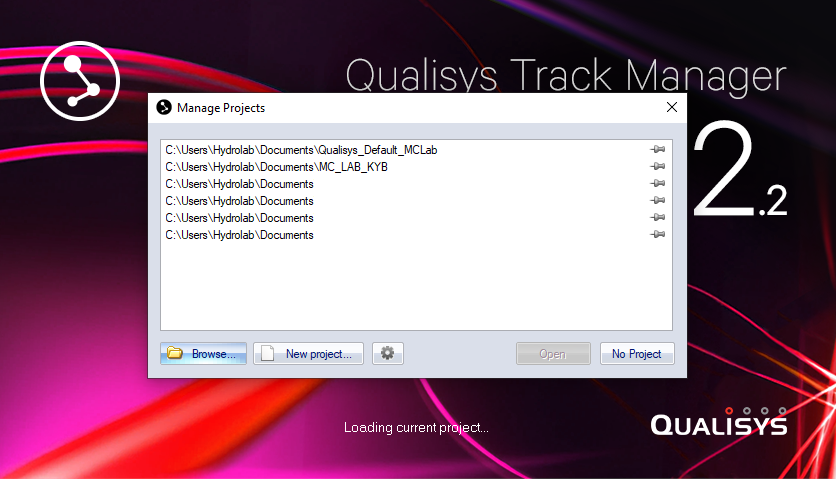
\includegraphics[width=0.5\textwidth]{QTM/01_manage_projects_window}
		\caption{The first window that appears when starting QTM. Here you will select your project or create a new one}
		\label{fig:manageprojects}
	\end{figure}
	
	\begin{figure}[H]
		\centering
		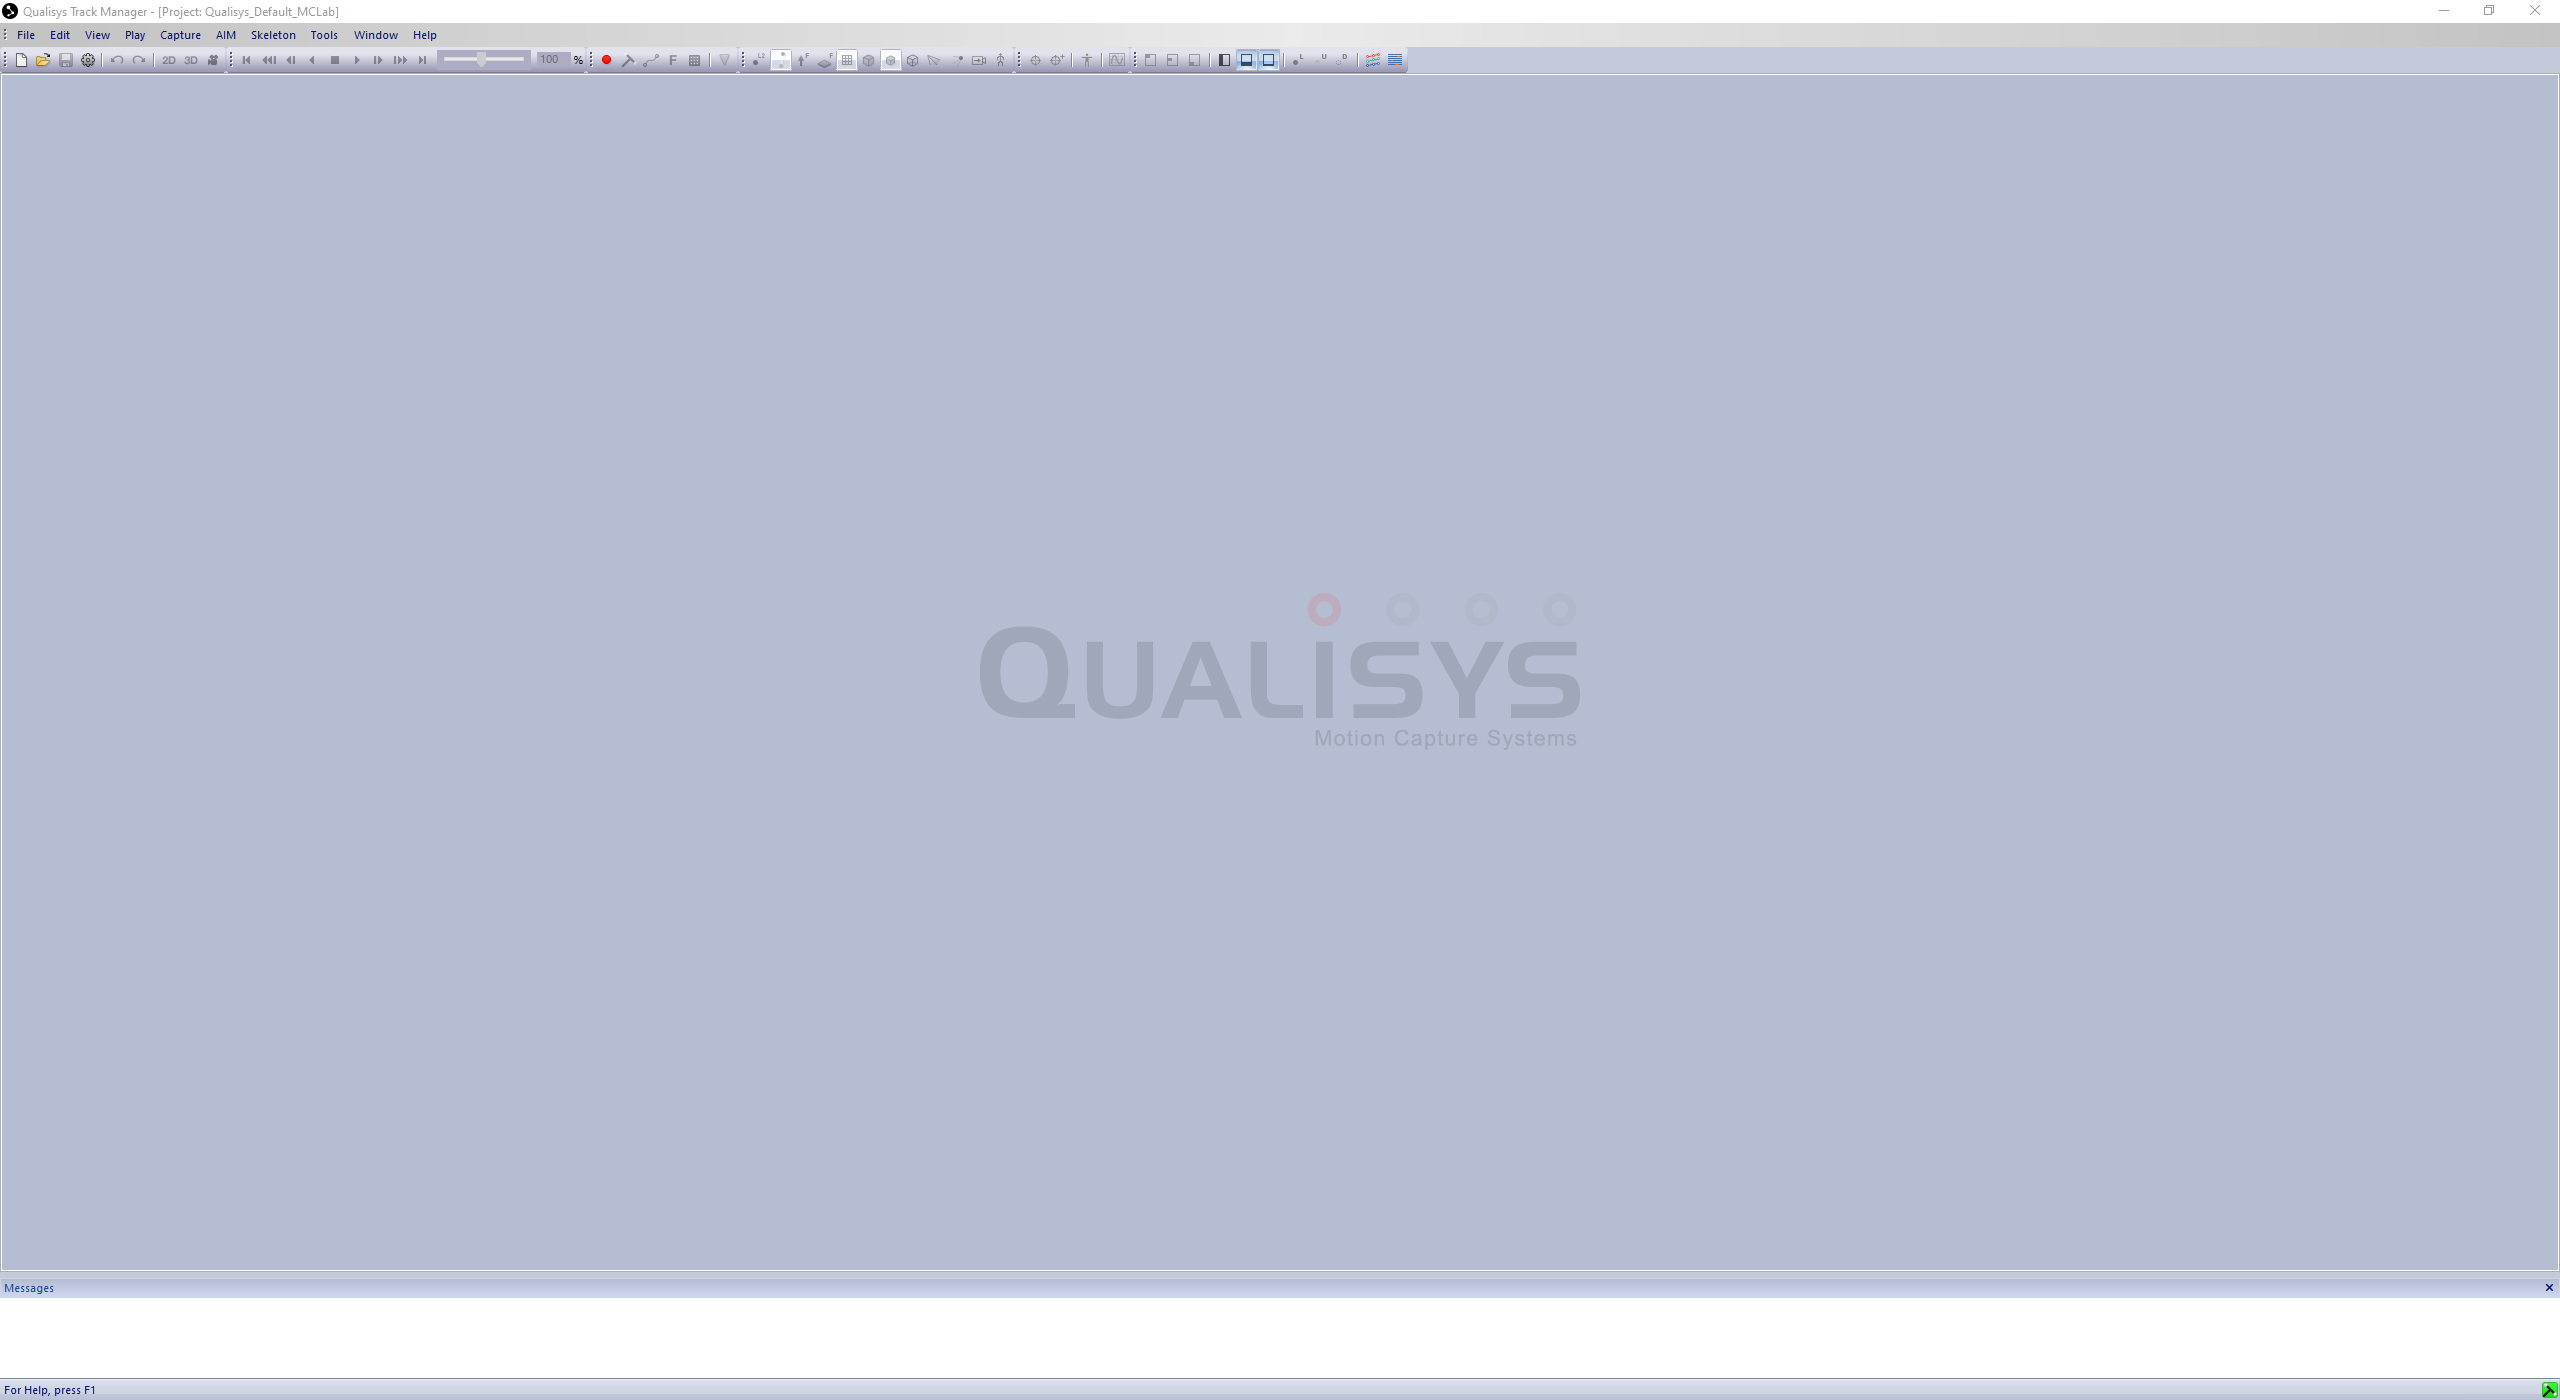
\includegraphics[width=0.5\textwidth]{QTM/02_new_measurement_window}
		\caption{Start a new measurement window by clicking the white sheet in the top left or pressing \texttt{CTRL + N}. You must also repeat this if the qualisys system crashes.}
		\label{fig:MeasurmentWindow}
	\end{figure}
	
	\begin{figure}[H]
		\centering
		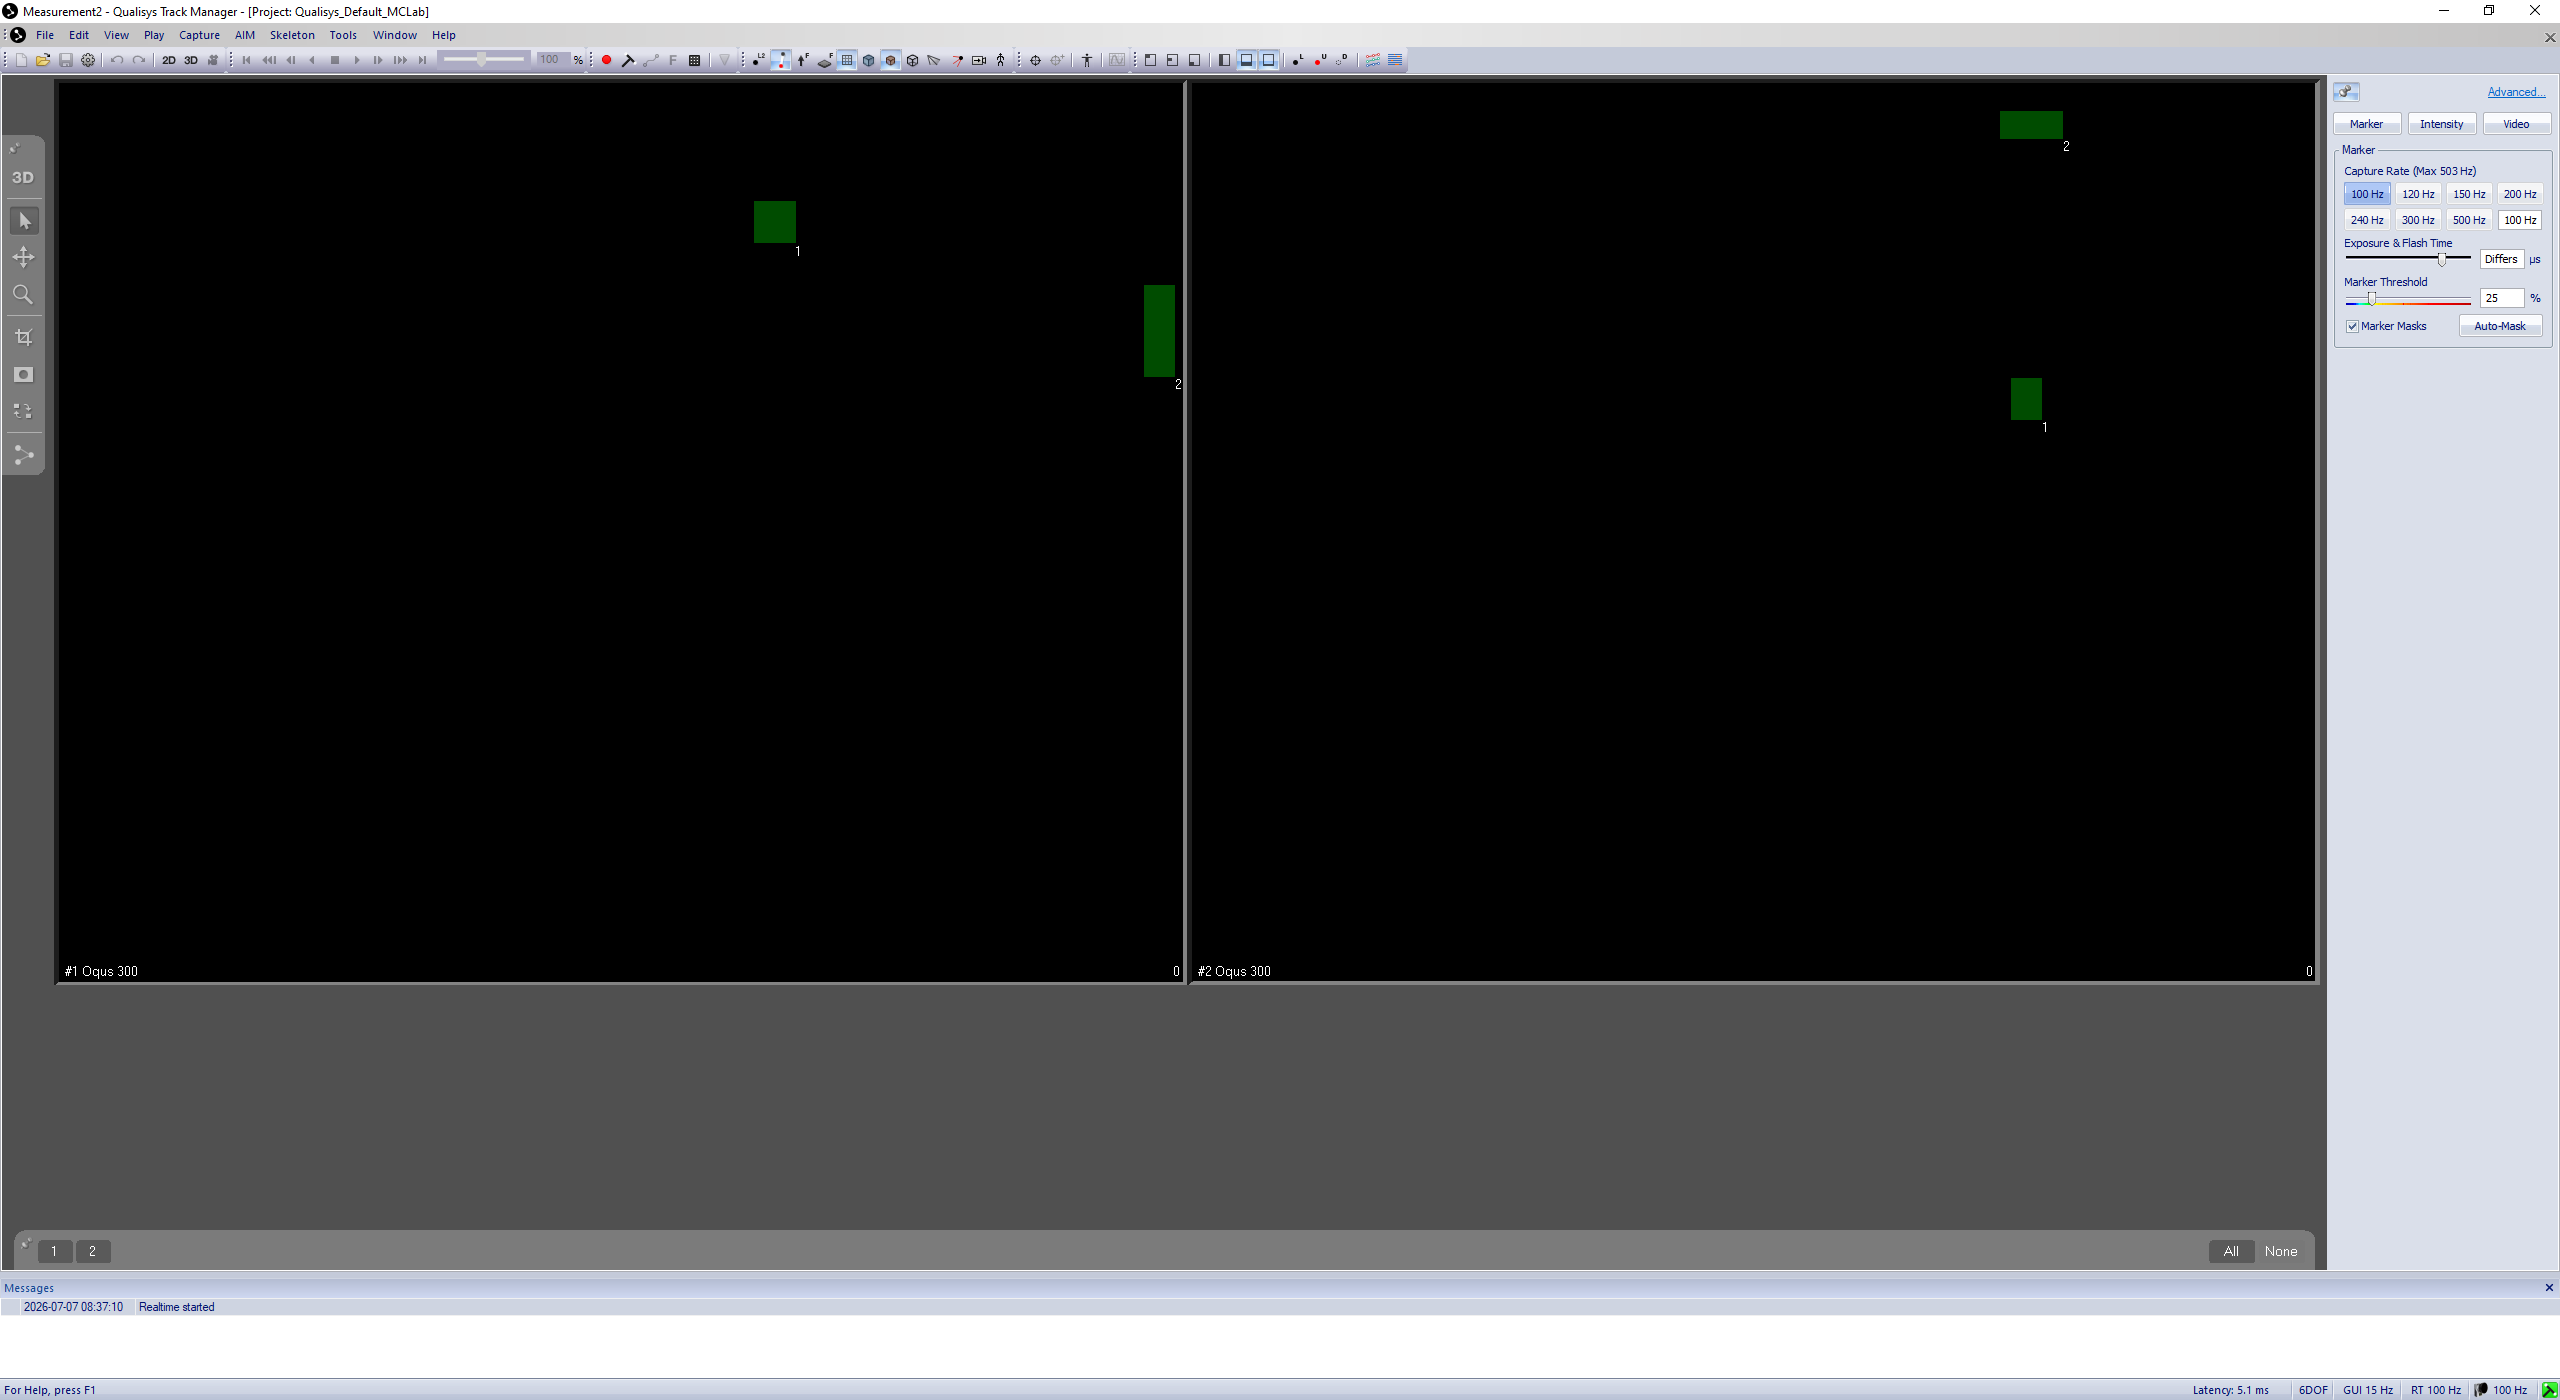
\includegraphics[width=0.5\textwidth]{QTM/03_camera_view_marker_mode}
		\caption{Camera view in \textit{marker mode} click on the \textit{3D} icon on the left to enter \textit{3D mode}.}
		\label{fig:Cameraview}
	\end{figure}
	
	\begin{figure}[H]
		\centering
		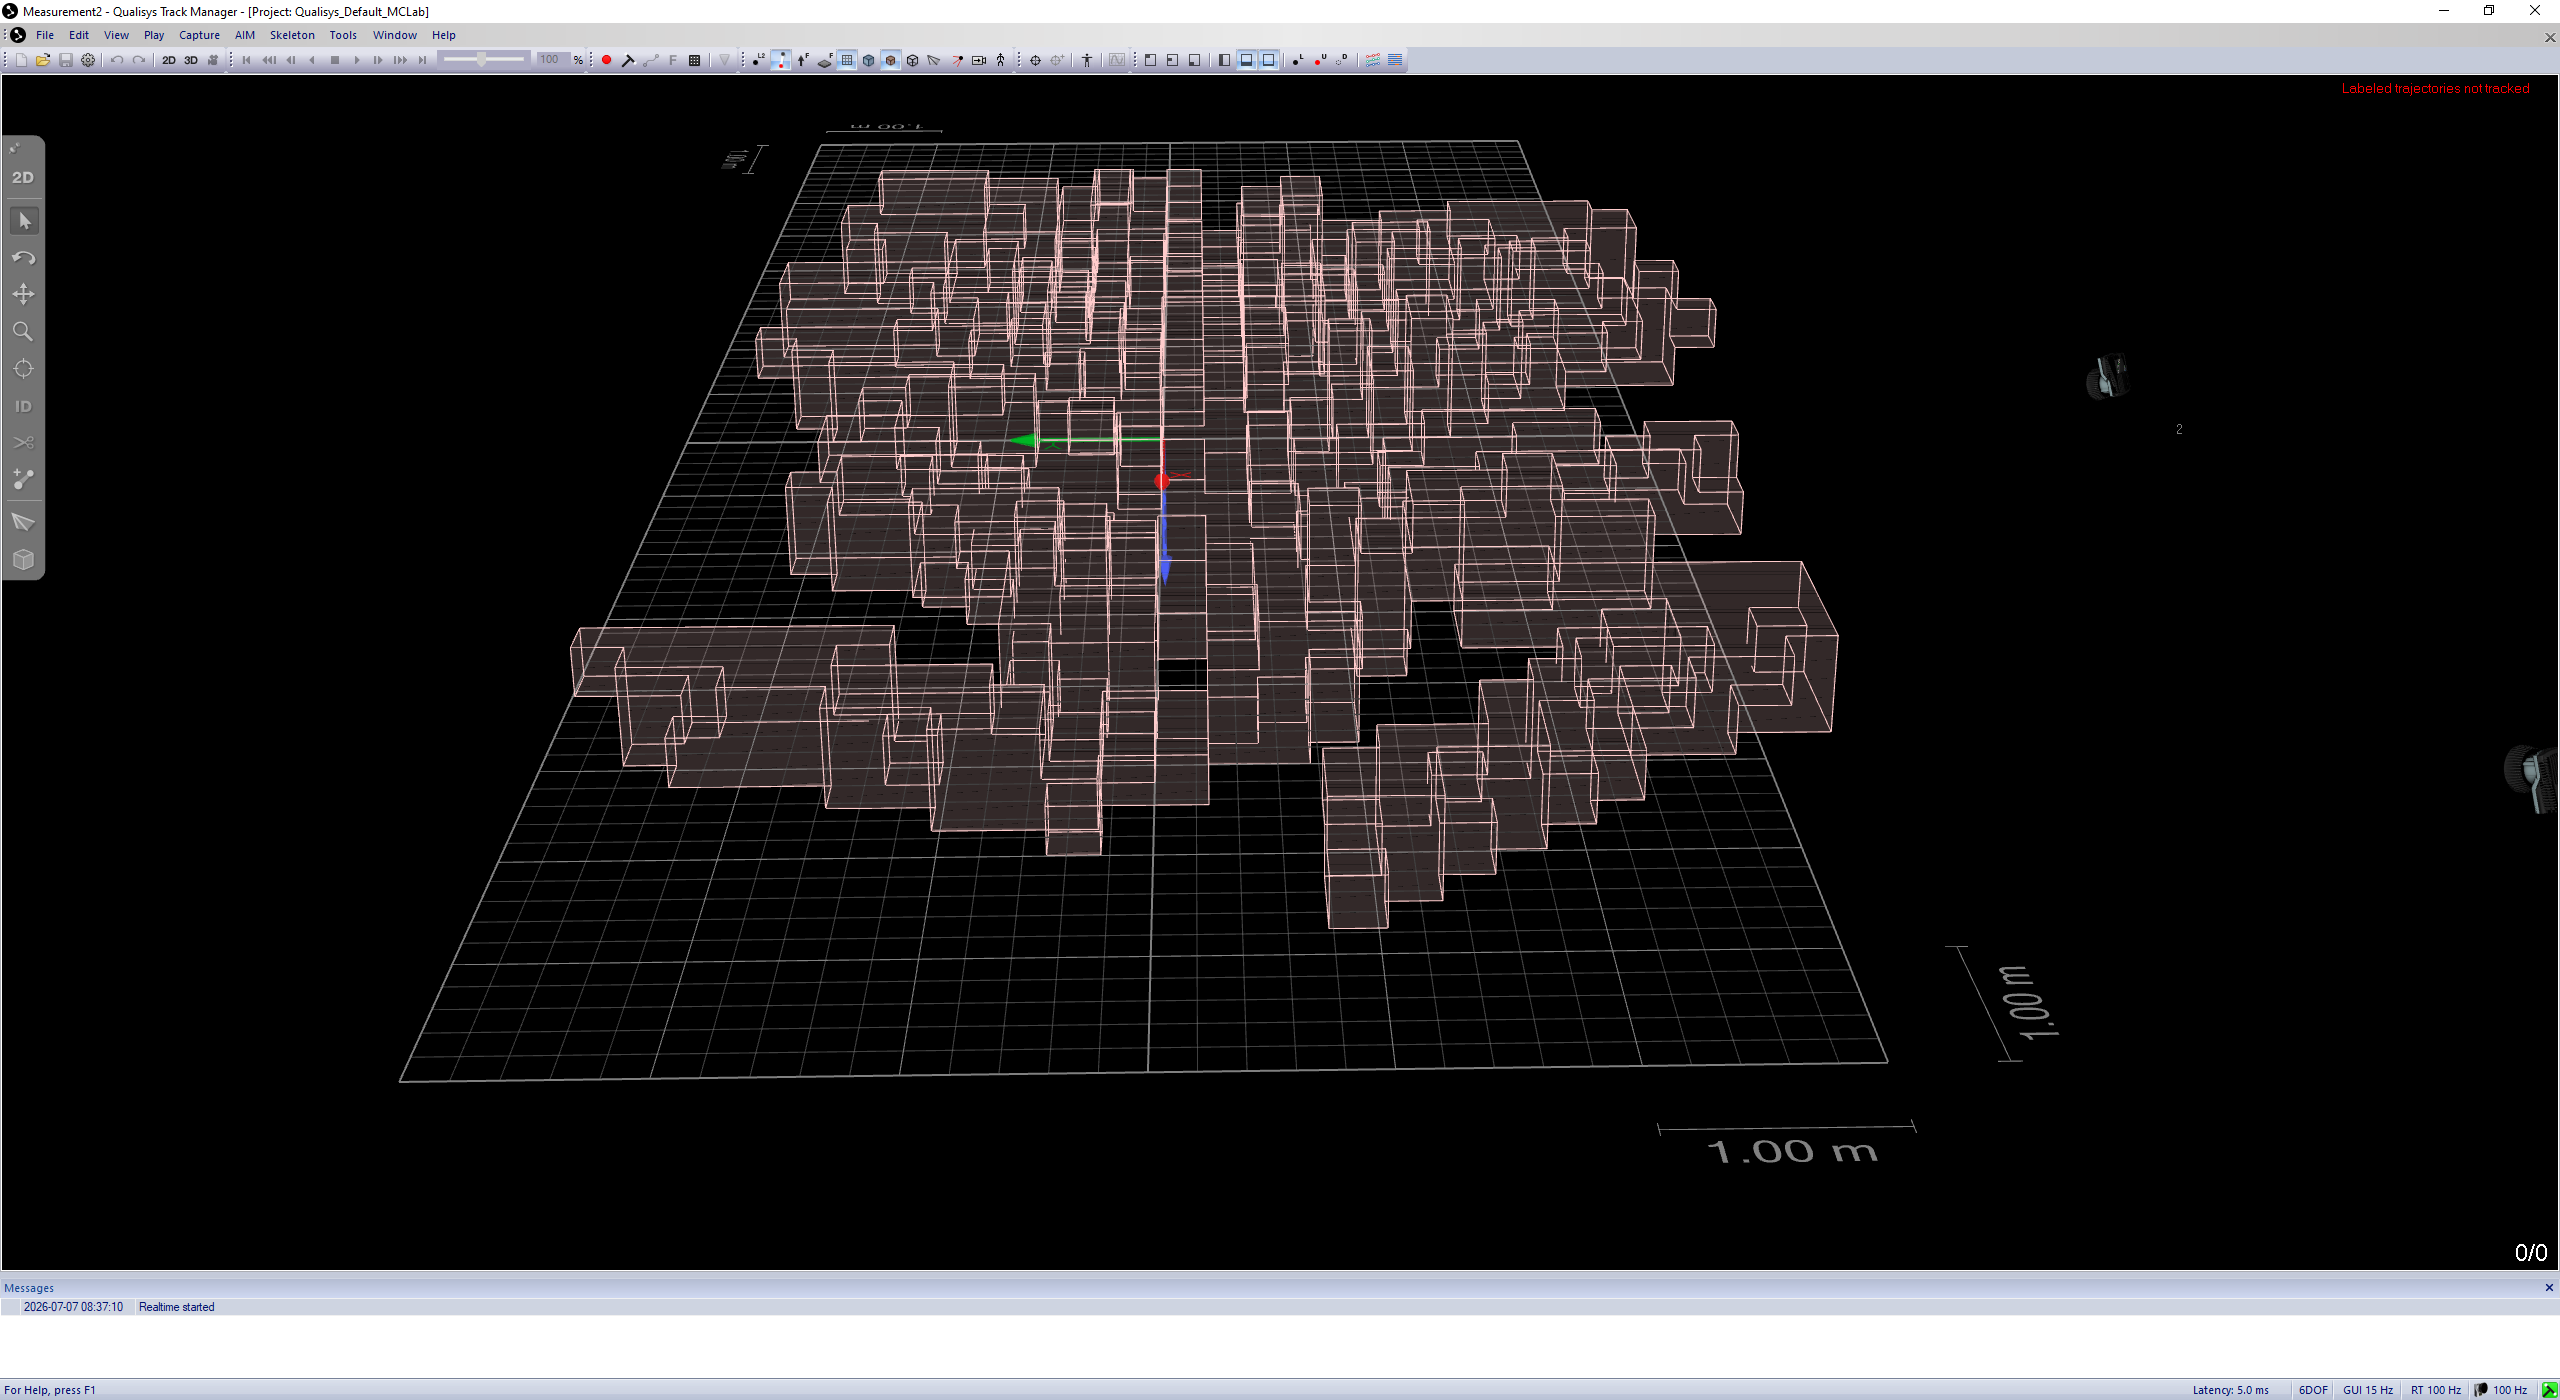
\includegraphics[width=0.5\textwidth]{QTM/04_lab_frame_calibrated_volume}
		\caption{Lab frame of reference with the calibrated volume shown. Press \texttt{CTRL + D} or alternatively click \textit{view} on the top toolbar and then select \textit{Data Info 1} to show marker positions in \textit{2D}.}
		\label{fig:labFrame}
	\end{figure}
	
	\begin{figure}[H]
		\centering
		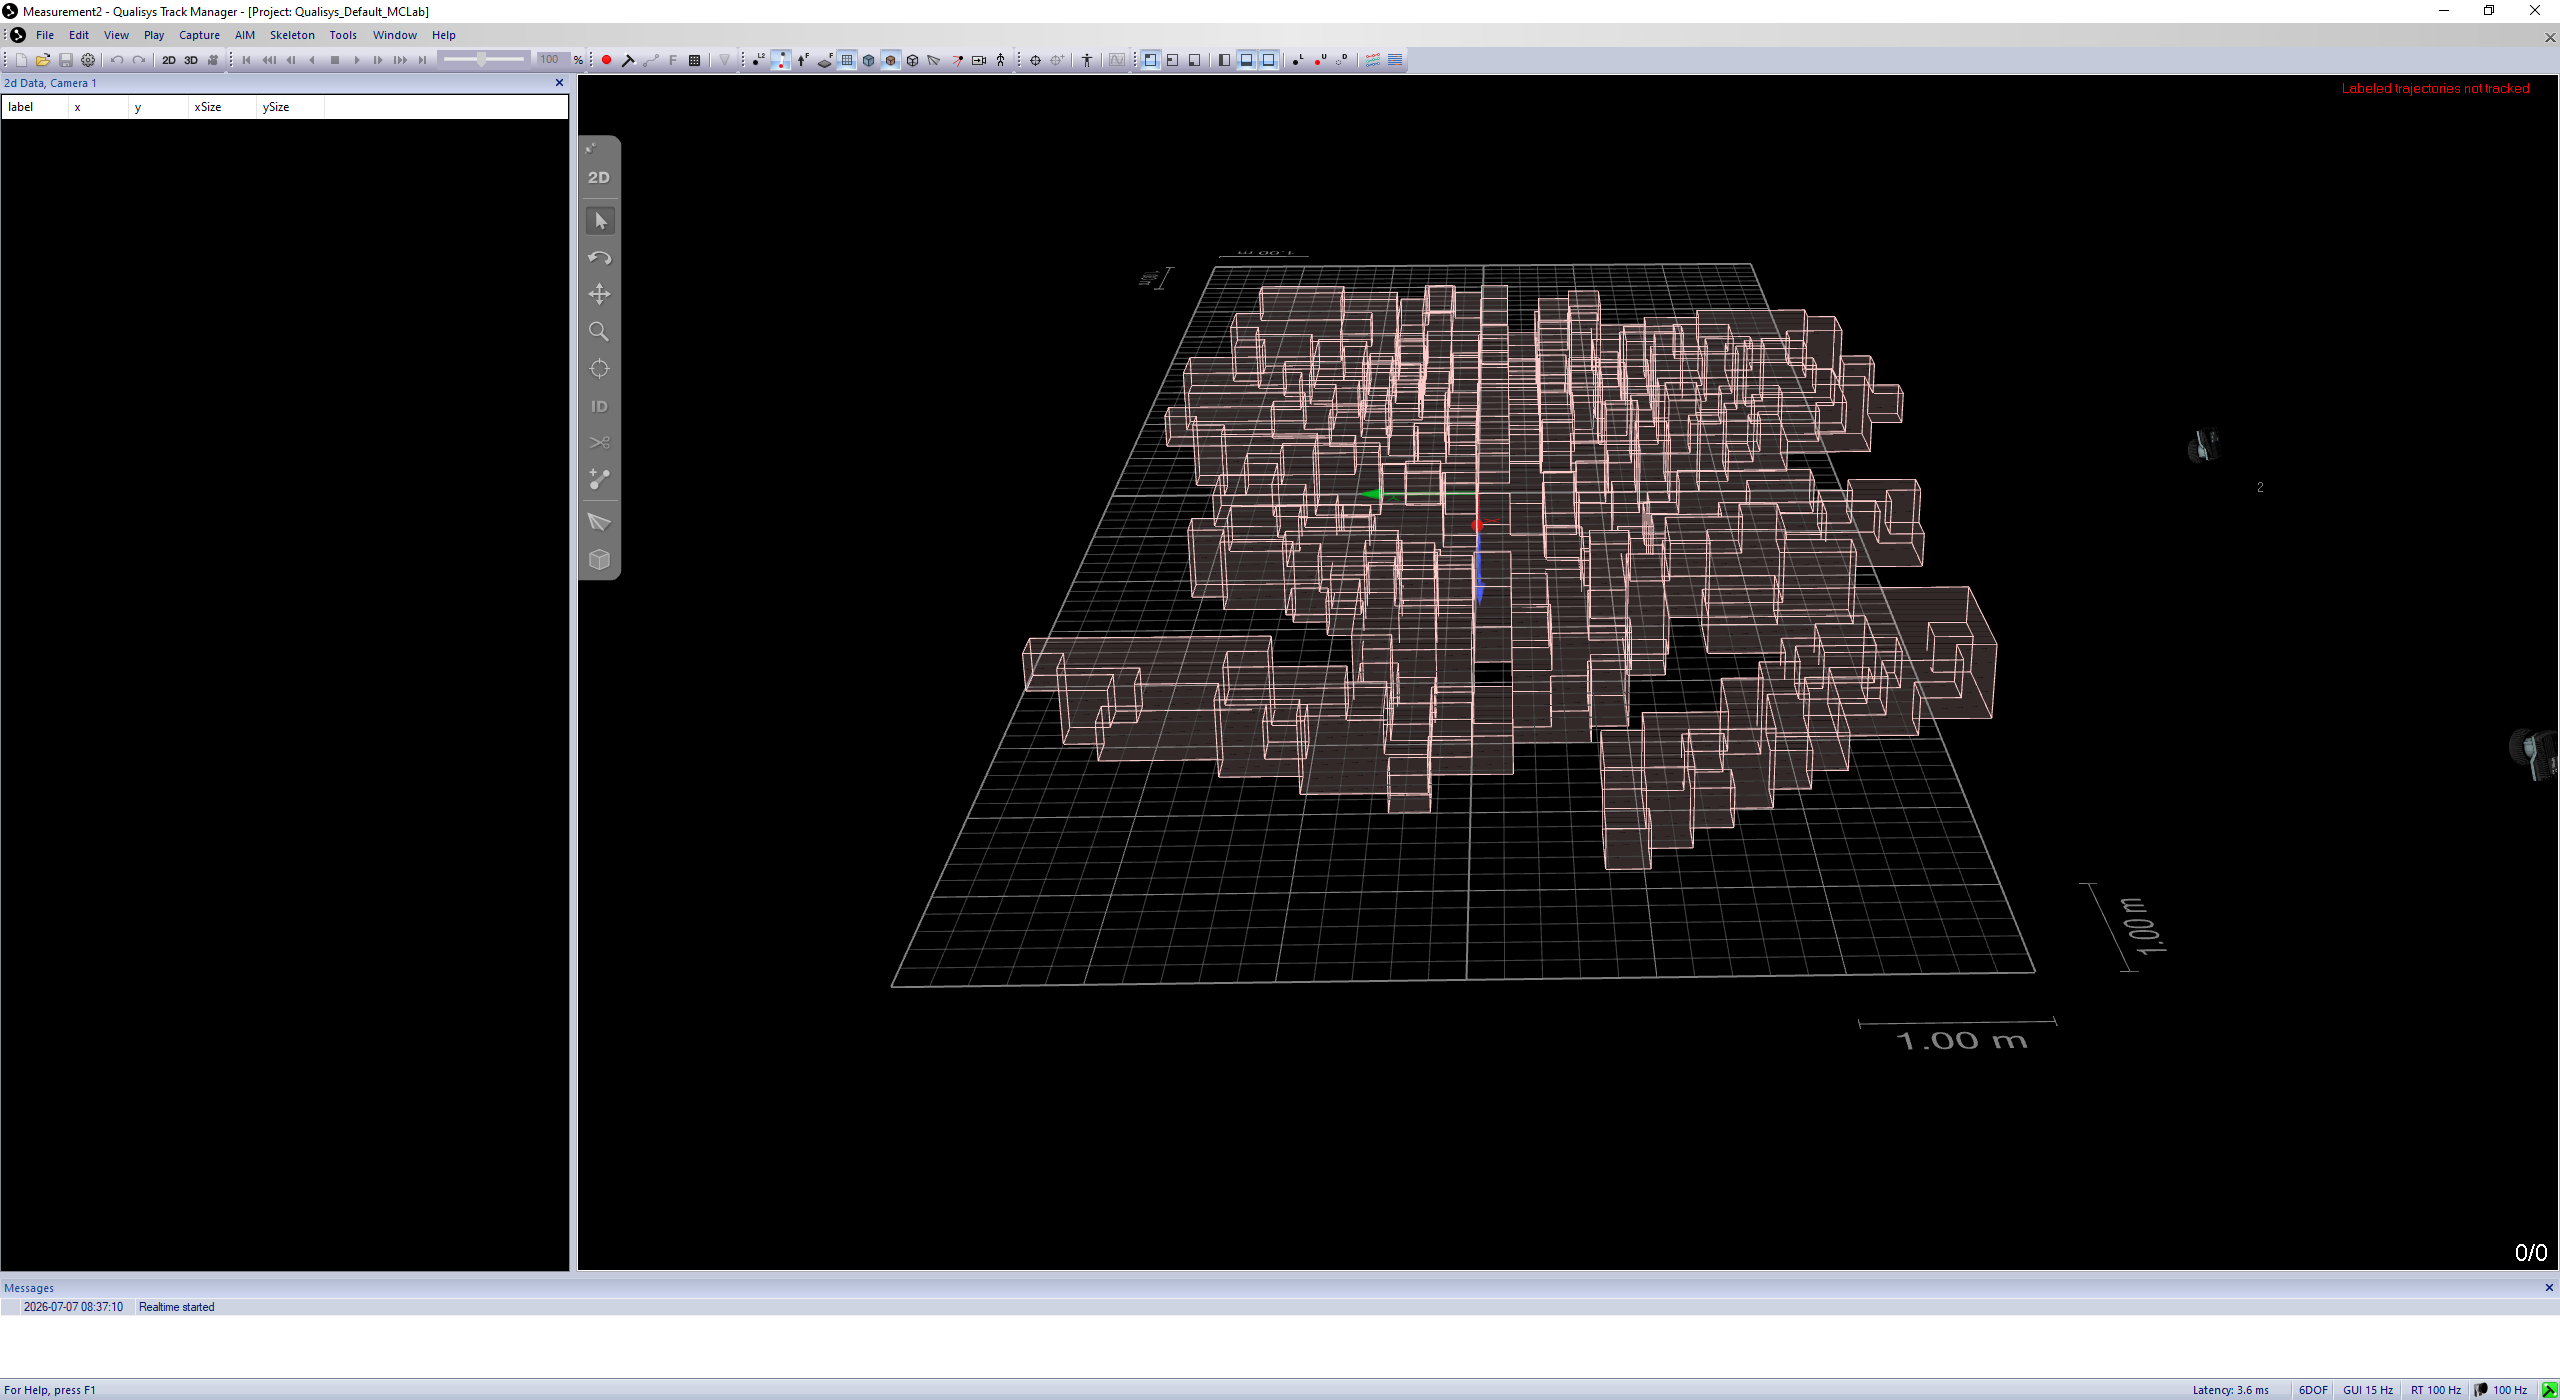
\includegraphics[width=0.5\textwidth]{QTM/05_lab_frame_marker_coordinates}
		\caption{Lab frame of reference with the calibrated volume and 2D marker position shown. Right click and select \textit{6DOF} to show rigid body coordinates.}
		\label{fig:3D}
	\end{figure}
	
	\begin{figure}[H]
		\centering
		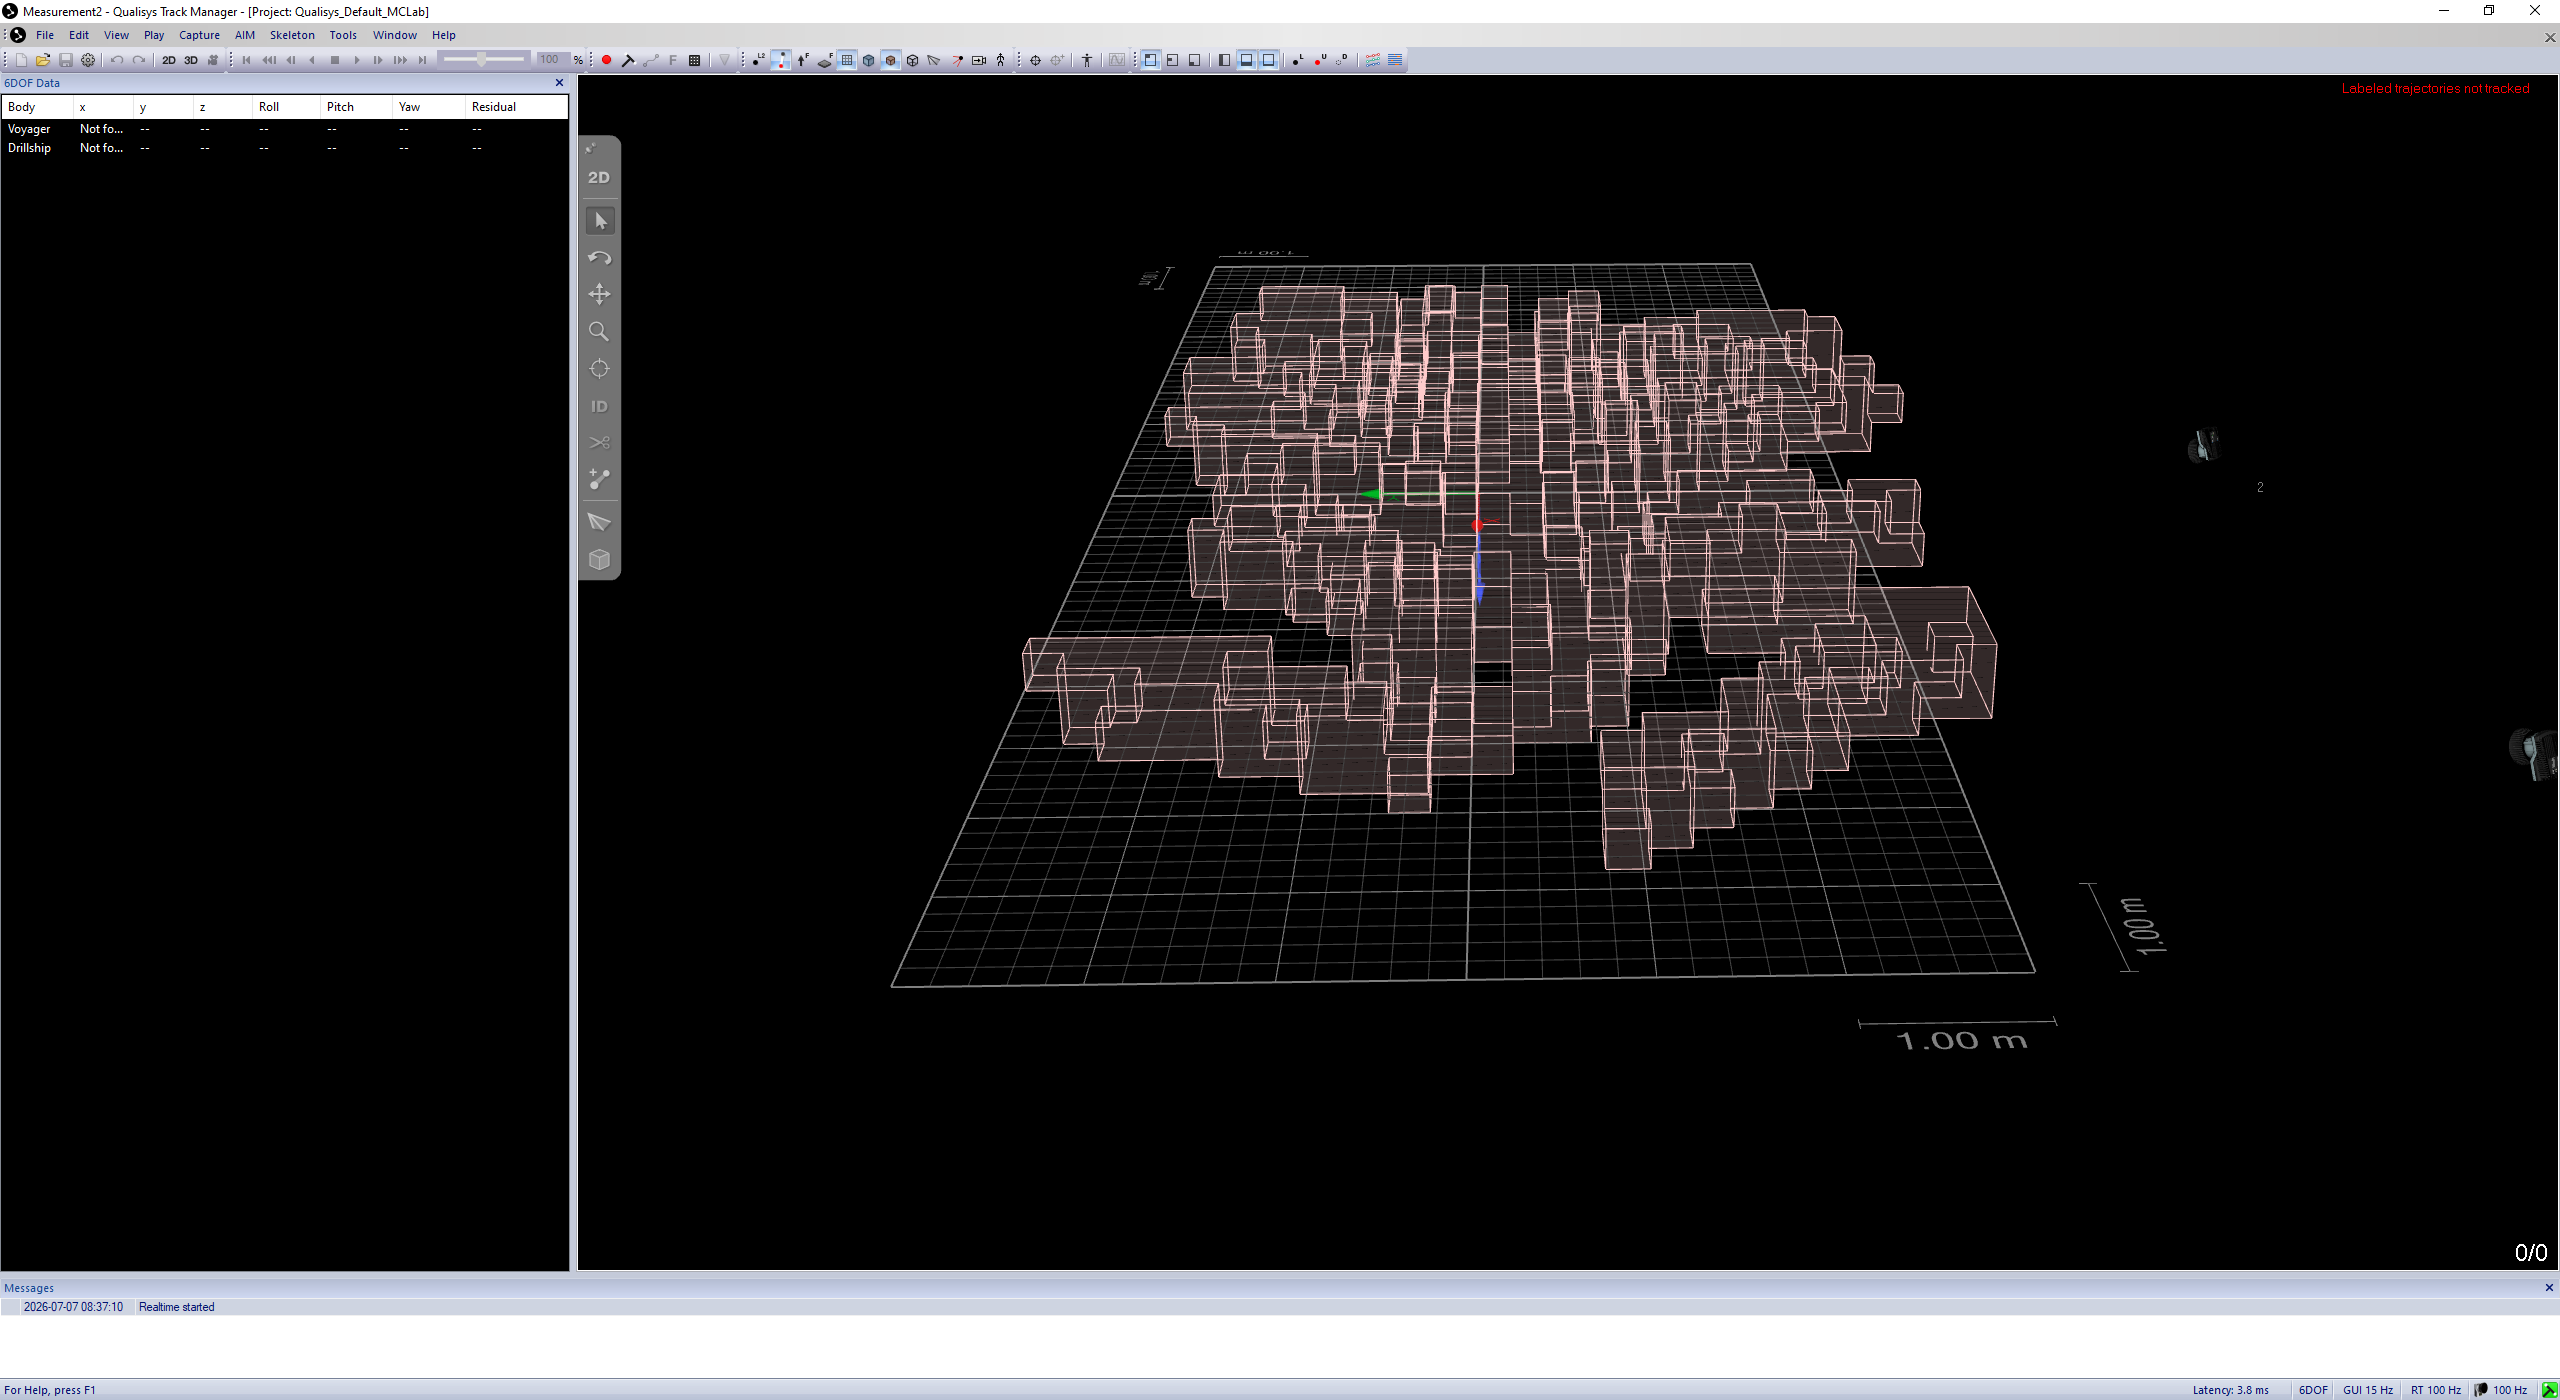
\includegraphics[width=0.5\textwidth]{QTM/06_lab_frame_6dof_coordinates}
		\caption{Lab frame of reference with the calibrated volume and rigid body coordinates.}
		\label{fig:6DOF}
	\end{figure}
	
	\begin{figure}[H]
		\centering
		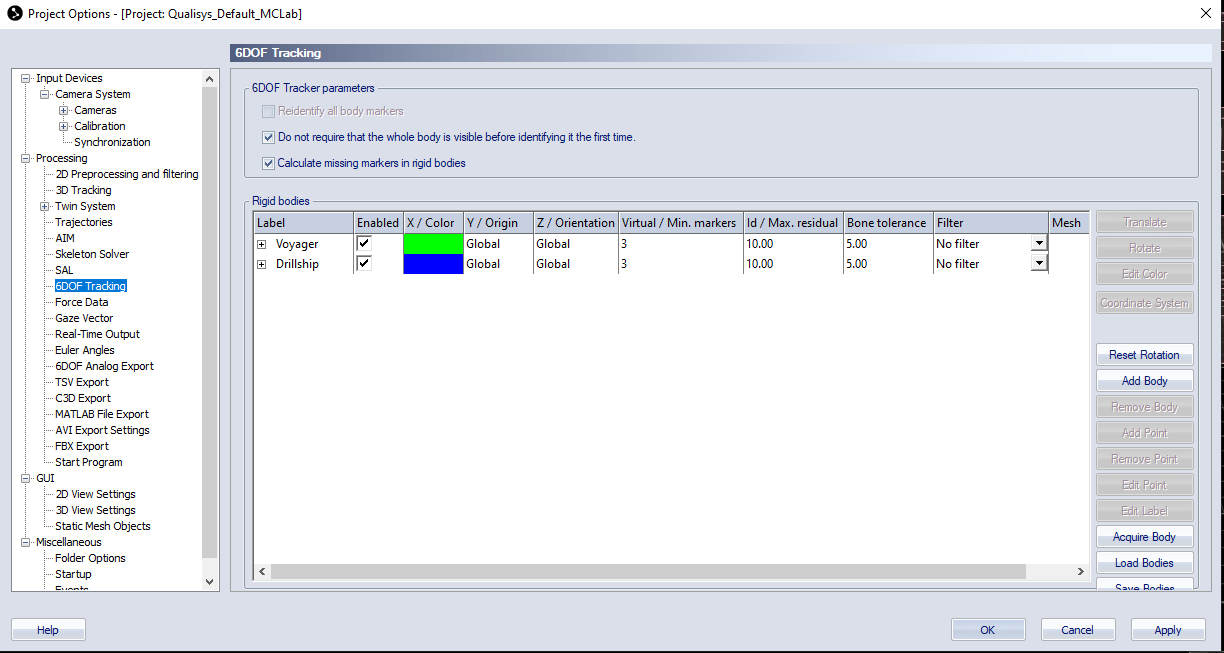
\includegraphics[width=0.5\textwidth]{QTM/07_6dof_tracking_settings}
		\caption{\textit{6DOF Settings} window were you can \textit{Add}, \textit{Acquire}, \textit{Load}, and \textit{Save} rigid bodies.}
		\label{fig:6DOFSettings}
	\end{figure}
	
	
	\begin{figure}[H]
		\centering
		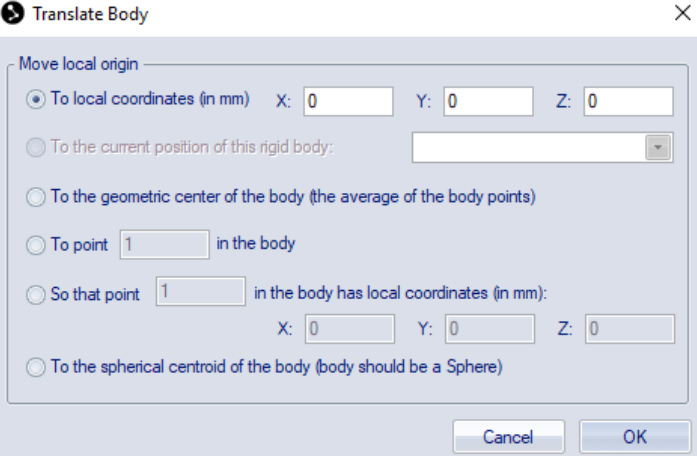
\includegraphics[width=0.5\textwidth]{QTM/08_translate_body_settings}
		\caption{\emph{Translate Body} Settings where we can move the local origin.}
		\label{fig:6DOFSettings_translate}
	\end{figure}
	
	% Visual references for correct setup and common issues
	
	% ============================================================
	\section{Thruster System}
	\label{sec:thrusters}
	% ============================================================
	
	The \texttt{cybership\_thrusters} package implements low-level thruster drivers in C++. It
	supports three actuator types.
	
	\subsection{Thruster Types}
	
	\begin{description}[leftmargin=2.5cm]
		\item[VSP] \textit{Voith Schneider Propeller} -- Outputs differential arm positions
		(\texttt{arm\_x}, \texttt{arm\_y}) and a fixed RPM command. Suitable for omnidirectional
		propulsion.
		\item[Fixed] A single-axis thruster outputting a normalized force signal. Force is linearly
		interpolated between \texttt{force\_min} and \texttt{force\_max}.
		\item[Azimuth] Computes both a rotation angle (via \texttt{atan2}) and an RPM from the
		magnitude of the input force vector. Used for azimuth-steerable pods.
	\end{description}
	
	\subsection{Safety Watchdog}
	
	All thruster controllers include a watchdog timer. If no force command is received on the
	configured \texttt{force\_topic} within \textbf{2.0~seconds} (configurable per thruster), the
	driver automatically publishes zero on all output topics. The watchdog runs at 10~Hz.
	
	\subsection{Enabling / Disabling Thrusters}
	
	Thrusters are \textbf{disabled by default}. They must be explicitly enabled via ROS~2 service
	call:
	
	\begin{lstlisting}[style=bash]
		# Enable
		ros2 service call <vessel_name>/thruster/enable std_srvs/srv/Empty {}
		
		# Disable
		ros2 service call <vessel_name>/thruster/disable std_srvs/srv/Empty {}
	\end{lstlisting}
	
	\textbf{Operational note}: Before handing control to students, always navigate to the thrust
	allocation web UI at \texttt{http://192.168.1.102:8001} and \textbf{deactivate the thrust
		allocation} until the student controller is ready.
	
	\subsection{Thruster Configuration (YAML)}
	
	Thrusters are configured under the \texttt{thrusters} namespace in a YAML parameter file.
	Each thruster has a unique name and a type-specific set of parameters:
	
	\begin{lstlisting}[style=yaml]
		thrusters:
		bow_thruster:
		type: "fixed"
		force_topic: "/voyager/bow_thruster/force"
		signal_topic: "/voyager/bow_thruster/signal"
		force_max: 5.0
		force_min: -5.0
		signal_inverted: false
		safety_timeout: 2.0
		
		port_azimuth:
		type: "azimuth"
		force_topic: "/voyager/port_azimuth/force"
		angle_topic: "/voyager/port_azimuth/angle"
		rpm_topic: "/voyager/port_azimuth/rpm"
		force_max: 20.0
		force_min: -20.0
		angle_inverted: false
		rpm_inverted: false
		
		vsp_main:
		type: "vsp"
		force_topic: "/voyager/vsp/force"
		arm_x_topic: "/voyager/vsp/arm_x"
		arm_y_topic: "/voyager/vsp/arm_y"
		rpm_topic: "/voyager/vsp/rpm"
		force_max: 10.0
		force_min: -10.0
		rpm_cmd: 1000.0
		arm_x_inverted: false
		arm_y_inverted: false
	\end{lstlisting}
	
	% ============================================================
	\section{Dynamic Positioning}
	\label{sec:dp}
	% ============================================================
	
	The \texttt{cybership\_dp} package implements two layered controllers for dynamic positioning.
	
	\subsection{Velocity Controller}
	
	The velocity controller receives a desired velocity setpoint and computes force/torque demands
	using independent PID loops for surge, sway, and yaw. Gains are specified in the package's
	\texttt{config/} YAML files. Computed demands are published to the force controller.
	
	\subsection{Force Controller}
	
	The force controller uses the \textbf{Skadi} library
	(\url{https://github.com/incebellipipo/skadipy}) for optimal thrust allocation. It receives
	3-DOF force/torque demands (surge, sway, yaw) and distributes them across the available
	thrusters.
	
	\subsection{Launch Files}
	
	\begin{lstlisting}[style=bash]
		# Full DP system (velocity + force controller)
		ros2 launch cybership_dp dp.launch.py \
		vessel_name:=voyager vessel_model:=voyager
		
		# Force controller only
		ros2 launch cybership_dp force_controller.launch.py \
		vessel_name:=voyager vessel_model:=voyager
		
		# Velocity controller only
		ros2 launch cybership_dp velocity_controller.launch.py \
		vessel_name:=voyager vessel_model:=voyager
	\end{lstlisting}
	
	\subsection{Vessel Model Support}
	
	The \texttt{voyager} model is fully supported. Support for \texttt{enterprise} and
	\texttt{drillship} is planned but not yet complete.
	
	% ============================================================
	\section{Simulation}
	\label{sec:simulation}
	% ============================================================
	
	The \texttt{cybership\_simulator} package provides lightweight Python scripts that simulate
	vessel dynamics using simplified physics. Each vessel has its own dedicated script, currently
	including:
	
	\begin{itemize}
		\item CyberShip Enterprise~1 (3-DOF planar model)
	\end{itemize}
	
	The simulator publishes the same topics as the physical bringup stack (odometry, transforms)
	so that all higher-level control packages are compatible with both modes.
	
	Pass \texttt{use\_sim\_time:=true} to any launch file when running in simulation:
	
	\begin{lstlisting}[style=bash]
		ros2 launch cybership_bringup voyager.launch.py \
		vessel_name:=voyager vessel_model:=voyager \
		use_sim_time:=true
	\end{lstlisting}
	
	% ============================================================
	\section{Visualization}
	\label{sec:visualization}
	% ============================================================
	
	\subsection{RViz}
	
	The \texttt{cybership\_viz} package provides preconfigured RViz scenes showing:
	
	\begin{itemize}
		\item The vessel URDF model with live TF transforms.
		\item Sensor data overlays (IMU, pose estimates).
		\item Trajectory history.
	\end{itemize}
	
	\subsection{URDF / Robot State Publisher}
	
	The vessel's 3D model is published by the \texttt{robot\_state\_publisher} node. URDF files
	and mesh assets live in \texttt{cybership\_description/urdf/} and
	\texttt{cybership\_description/meshes/} respectively. To launch standalone visualization:
	
	\begin{lstlisting}[style=bash]
		ros2 launch cybership_description description.launch.py
	\end{lstlisting}
	
	\subsection{Utilities Web UI}
	
	A lightweight web interface runs on the master node and is accessible at:
	
	\begin{center}
		\url{http://192.168.1.102:8001}
	\end{center}
	
	It can be started with:
	
	\begin{lstlisting}[style=bash]
		ros2 launch cybership_utilities ui.launch.py
	\end{lstlisting}
	
	\subsection{Force Mux GUI}
	
	The \texttt{cybership\_utilities} package also includes a PyQt GUI
	(\texttt{nodes/force\_mux\_gui.py}) for inspecting and switching the active force-mux input
	topic for a selected vessel namespace. The namespace can be supplied via the
	\texttt{VEHICLE\_NS} environment variable or typed directly in the GUI.
	
	% ============================================================
	\section{Joystick / Teleoperation}
	\label{sec:teleop}
	% ============================================================
	
	Bluetooth joysticks are connected to the master node using \texttt{bluetoothctl}. Once
	connected, the teleop stack is launched with:
	
	\begin{lstlisting}[style=bash]
		# Drillship on joystick 0
		ros2 launch cybership_teleop allocation.launch.py \
		vessel_name:=drillship joy_id:=0
		
		# Voyager on joystick 1
		ros2 launch cybership_teleop allocation.launch.py \
		vessel_name:=voyager joy_id:=1
	\end{lstlisting}
	
	Raw joystick events are published by the standard \texttt{joy} node:
	
	\begin{lstlisting}[style=bash]
		ros2 run joy joy_node
	\end{lstlisting}
	
	% ============================================================
	\section{ROS~2 Interfaces}
	\label{sec:interfaces}
	% ============================================================
	
	The \texttt{cybership\_interfaces} package defines the custom ROS~2 interfaces used across the
	suite. Currently defined interfaces are listed in Table~\ref{tab:interfaces}.
	
	\begin{table}[ht]
		\centering
		\begin{tabular}{llp{7cm}}
			\toprule
			\textbf{Type} & \textbf{Name}           & \textbf{Description}                     \\
			\midrule
			Service       & \texttt{ResetSimulator} & Resets the simulator to a given 2D pose.
			Request: \texttt{geometry\_msgs/Pose2D}.
			Response: \texttt{bool success}.                                                   \\
			\bottomrule
		\end{tabular}
		\caption{Custom ROS~2 interfaces.}
		\label{tab:interfaces}
	\end{table}
	
	To depend on these interfaces from another package:
	
	\begin{lstlisting}[style=bash,language=XML]
		<!-- package.xml -->
		<depend>cybership_interfaces</depend>
	\end{lstlisting}
	
	\begin{lstlisting}[style=bash]
		# Python usage
		from cybership_interfaces.srv import ResetSimulator
	\end{lstlisting}
	
	% ============================================================
	\section{External Dependencies}
	\label{sec:external}
	% ============================================================
	
	Third-party packages are included as Git submodules under \texttt{cybership\_external/}.
	Table~\ref{tab:external} lists each dependency.
	
	\begin{table}[ht]
		\centering
		\begin{tabular}{lp{9cm}}
			\toprule
			\textbf{Package}                    & \textbf{Description}                                                     \\
			\midrule
			\texttt{mocap4ros2\_qualisys}       & ROS~2 driver for the Qualisys optical motion capture system.             \\
			\texttt{dynamixel\_azimuth\_driver} & ROS~2 driver for Dynamixel motors used as azimuth actuators.             \\
			\texttt{ros2\_pca9685}              & ROS~2 driver for the PCA9685 I\textsuperscript{2}C PWM controller board. \\
			\texttt{mocap4r2\_msgs}             & ROS~2 message definitions for motion capture data.                       \\
			\texttt{bno055}                     & ROS~2 driver for the Bosch BNO055 9-axis IMU.                            \\
			\bottomrule
		\end{tabular}
		\caption{External submodule dependencies.}
		\label{tab:external}
	\end{table}
	
	To update all submodules to their latest upstream versions:
	
	\begin{lstlisting}[style=bash]
		git submodule update --remote
	\end{lstlisting}
	
	% ============================================================
	\section{Configuration Reference}
	\label{sec:config}
	% ============================================================
	
	\subsection{Centralized Configuration}
	
	The \texttt{cybership\_config} package stores YAML configuration files that are installed and
	shared across the suite. Vessel-specific overrides are placed in per-vessel subdirectories
	within \texttt{config/}.
	
	\subsection{Common Launch Arguments}
	
	The \texttt{cybership\_utilities} package defines a set of standardized launch arguments used
	by all launch files:
	
	\begin{description}[leftmargin=3.5cm]
		\item[\texttt{vessel\_model}] Model identifier string (e.g., \texttt{voyager},
		\texttt{enterprise}, \texttt{drillship}).
		\item[\texttt{vessel\_name}] ROS~2 namespace for the vessel (typically matches
		\texttt{vessel\_model}).
		\item[\texttt{param\_file}] Path to an optional override parameter file.
		\item[\texttt{use\_sim\_time}] Boolean flag to use simulation time clock.
	\end{description}
	
	\subsection{ROS Environment}
	
	The vessel's ROS setup script is located at \texttt{\textasciitilde/.rosrc}. Source it
	before running ROS~2 commands on the vessel:
	
	\begin{lstlisting}[style=bash]
		source ~/.rosrc
	\end{lstlisting}
	
	% ============================================================
	\section{Systemd Service Management}
	\label{sec:systemd}
	% ============================================================
	
	Vessel bringup and the Fast~DDS discovery server are managed as \textbf{systemd user services}.
	
	\begin{description}[leftmargin=5cm, style=nextline]
		\item[\texttt{ros2-cybership-<model>}] Per-vessel bringup service. Starts automatically at
		boot on the corresponding Raspberry Pi.
		\item[FastDDS service] Runs on \texttt{cybership-master} as a user service, providing the
		DDS discovery server on port~11811.
	\end{description}
	
	Useful service management commands:
	
	\begin{lstlisting}[style=bash]
		# Check status
		systemctl --user status ros2-cybership-voyager
		
		# Restart bringup
		systemctl --user restart ros2-cybership-voyager
		
		# View logs
		journalctl --user -u ros2-cybership-voyager -f
	\end{lstlisting}
	
	% ============================================================
	\section{Operational Procedure}
	\label{sec:operations}
	% ============================================================
	
	\subsection{Standard Startup Sequence}
	
	\begin{enumerate}
		\item Power the vessel by connecting the battery. The bringup service starts automatically.
		\item On the control workstation, ensure the ROS discovery server variables are set in
		\texttt{\textasciitilde/.bashrc} (Section~\ref{sec:network}) and restart the daemon.
		\item Open the web UI at \texttt{http://192.168.1.102:8001} and
		\textbf{deactivate the thrust allocation}.
		\item Wait for the EKF to converge (monitor covariance on
		\texttt{/<vessel\_name>/measurement/odom} or watch RViz).
		\item Once the student controller is ready, re-enable thrust allocation from the web UI or
		via the service call.
		\item Keep the vessel within the motion-capture calibrated area during experiments.
	\end{enumerate}
	
	\subsection{Troubleshooting}
	
	\begin{description}[leftmargin=4cm, style=nextline]
		\item[Topics not visible] Restart the ROS~2 daemon:
		\begin{lstlisting}[style=bash]
			ros2 daemon stop ; ros2 daemon start\end{lstlisting}
		\item[EKF diverging] Check the covariance on
		\texttt{/<vessel\_name>/measurement/odom}. Ensure the vessel is within the mocap
		calibrated area and that the Qualisys system has acquired all markers.
		\item[Rigid body order mismatch] Verify the rigid body order in the Qualisys software matches
		the expected vessel index. Order matters for index-based assignment.
		\item[Thrusters unresponsive] Confirm they are enabled:
		\begin{lstlisting}[style=bash]
			ros2 service call <vessel_name>/thruster/enable std_srvs/srv/Empty {}\end{lstlisting}
		Also verify no safety watchdog timeout has silenced the commands
		(check that force commands arrive within 2~s).
		\item[Discovery issues] Confirm the FastDDS service is running on
		\texttt{cybership-master} and that your workstation is on the
		\texttt{192.168.1.1/24} subnet.
	\end{description}
	
	% ============================================================
	\section{Developer Notes}
	\label{sec:dev}
	% ============================================================
	
	\subsection{Adding a New Vessel Model}
	
	\begin{enumerate}
		\item Add URDF and mesh files to \texttt{cybership\_description/urdf/} and
		\texttt{cybership\_description/meshes/}.
		\item Create a vessel-specific configuration directory under \texttt{cybership\_config/}.
		\item Add a new \texttt{<model>.launch.py} in \texttt{cybership\_bringup/launch/}.
		\item Register the model string in \texttt{cybership\_utilities/utilities.py}.
		\item Implement force and velocity controllers in \texttt{cybership\_dp/} for the new model.
	\end{enumerate}
	
	\subsection{Node Naming Convention}
	
	All nodes and topics are namespaced by the vessel name to allow multiple vessels on the same
	ROS~2 network without collisions:
	
	\begin{center}
		\texttt{/<vessel\_name>/<subsystem>/<topic>}
	\end{center}
	
	\subsection{Extending Interfaces}
	
	Custom messages and services should be added to \texttt{cybership\_interfaces}. After adding
	\texttt{.msg} or \texttt{.srv} files, update the \texttt{CMakeLists.txt} accordingly and
	rebuild the package.
	
	% ============================================================
	\section{Quick Operation Manual}
	\label{sec:quickops}
	% ============================================================
	
	This section is a concise step-by-step guide for the most common lab scenarios. For full
	explanations refer to the relevant sections of this document.
	
	% ------------------------------------------------------------
	\subsection{First-Time Workstation Setup}
	\label{ssec:first-time}
	% ------------------------------------------------------------
	
	Do this \textbf{once} on any computer that will interact with the vessels.
	
	\begin{enumerate}
		\item Connect to the lab Wi-Fi and confirm your IP is in \texttt{192.168.1.1/24}:
		\begin{lstlisting}[style=bash]
			ip addr
		\end{lstlisting}
		\item Add the following lines to \texttt{\textasciitilde/.bashrc}:
		\begin{lstlisting}[style=bash]
			export ROS_DISCOVERY_SERVER="192.168.1.102:11811"
			export ROS_SUPER_CLIENT=true
		\end{lstlisting}
		\item Apply the changes and restart the ROS~2 daemon:
		\begin{lstlisting}[style=bash]
			source ~/.bashrc
			ros2 daemon stop ; ros2 daemon start
		\end{lstlisting}
		\item Verify you can see ROS~2 topics from the network:
		\begin{lstlisting}[style=bash]
			ros2 topic list
		\end{lstlisting}
	\end{enumerate}
	
	% ------------------------------------------------------------
	\subsection{Starting an Experiment}
	\label{ssec:start-experiment}
	% ------------------------------------------------------------
	
	\begin{enumerate}
		\item \textbf{Power the vessel.} Connect the battery. The vessel boots and starts the ROS~2
		bringup automatically via systemd. No SSH needed.
		\item \textbf{Open the web UI} at \texttt{http://192.168.1.102:8001} and
		configure the vessel accoridng to your needs.
		\item \textbf{Wait for the EKF to converge.} Watch the vessel in RViz or check the
		covariance on the odometry topic:
		\begin{lstlisting}[style=bash]
			ros2 topic echo /voyager/measurement/odom
		\end{lstlisting}
		The diagonal elements of the covariance matrix should drop to small, stable values.
		\item \textbf{Ensure the vessel is inside the motion-capture calibrated area} before
		running any controller.
		\item \textbf{Launch the visualization} on your workstation (optional but recommended):
		\begin{lstlisting}[style=bash]
			ros2 launch cybership_utilities ui.launch.py
		\end{lstlisting}
	\end{enumerate}
	
	% ------------------------------------------------------------
	\subsection{Running a Student Controller}
	\label{ssec:student-controller}
	% ------------------------------------------------------------
	
	\begin{enumerate}
		\item Build and source the student package on the workstation:
		\begin{lstlisting}[style=bash]
			cd ~/ros_ws
			colcon build --packages-select <student_package>
			source install/setup.bash
		\end{lstlisting}
		\item Launch the student controller:
		\begin{lstlisting}[style=bash]
			ros2 launch <student_package> <launch_file>.launch.py \
			vessel_name:=voyager vessel_model:=voyager
		\end{lstlisting}
		\item Verify the controller is publishing on the expected force topic, then
		\textbf{activate} thrust allocation from the web UI at
		\texttt{http://192.168.1.102:8001}.
		\item Monitor the vessel. If behaviour is unexpected, immediately
		\textbf{deactivate} thrust allocation from the web UI.
	\end{enumerate}
	
	% ------------------------------------------------------------
	\subsection{Joystick Teleoperation}
	\label{ssec:joystick}
	% ------------------------------------------------------------
	
	\begin{enumerate}
		\item On \texttt{cybership-master}, connect the joystick via Bluetooth:
		\begin{lstlisting}[style=bash]
			bluetoothctl
			# Inside bluetoothctl:
			scan on
			pair <MAC>
			connect <MAC>
		\end{lstlisting}
		\item Launch the joy node and teleop allocator (on master or your workstation):
		\begin{lstlisting}[style=bash]
			ros2 run joy joy_node &
			ros2 launch cybership_teleop allocation.launch.py \
			vessel_name:=voyager joy_id:=1
		\end{lstlisting}
		\item Activate thrust allocation from the web UI and operate the vessel with the joystick.
	\end{enumerate}
	
	% ------------------------------------------------------------
	\subsection{Shutting Down}
	\label{ssec:shutdown}
	% ------------------------------------------------------------
	
	\begin{enumerate}
		\item Stop the student controller process (\texttt{Ctrl+C} in its terminal).
		\item Disconnect the vessel battery to power it off. The systemd service will stop cleanly.
		\item No further action is needed on \texttt{cybership-master}; it can be left running
		between sessions.
	\end{enumerate}
	
	% ------------------------------------------------------------
	\subsection{Restarting the Bringup on a Vessel}
	\label{ssec:restart-bringup}
	% ------------------------------------------------------------
	
	If the vessel bringup needs to be restarted (e.g.\ after a configuration change):
	
	\begin{lstlisting}[style=bash]
		ssh mclab@cybership-voyager.local
		systemctl --user restart ros2-cybership-voyager
		# Check it came back up:
		systemctl --user status ros2-cybership-voyager
	\end{lstlisting}
	
	% ============================================================
	\appendix
	\section{Quick-Reference Command Cheatsheet}
	\label{app:cheatsheet}
	% ============================================================
	
	\begin{lstlisting}[style=bash]
		## Environment setup (add to ~/.bashrc)
		export ROS_DISCOVERY_SERVER="192.168.1.102:11811"
		export ROS_SUPER_CLIENT=true
		
		## SSH
		ssh mclab@cybership-master.local
		ssh mclab@cybership-voyager.local
		ssh mclab@cybership-drillship.local
		
		## Vessel bringup (manual)
		ros2 launch cybership_bringup voyager.launch.py \
		vessel_name:=voyager vessel_model:=voyager
		
		## Utilities UI
		ros2 launch cybership_utilities ui.launch.py
		# Web UI: http://192.168.1.102:8001
		
		## Dynamic positioning
		ros2 launch cybership_dp dp.launch.py \
		vessel_name:=voyager vessel_model:=voyager
		
		## Teleop (joysticks)
		ros2 run joy joy_node
		ros2 launch cybership_teleop allocation.launch.py \
		vessel_name:=voyager joy_id:=1
		
		## Thrusters
		ros2 service call voyager/thruster/enable std_srvs/srv/Empty {}
		ros2 service call voyager/thruster/disable std_srvs/srv/Empty {}
		
		## Restart ROS daemon
		ros2 daemon stop ; ros2 daemon start
		
		## Monitor EKF
		ros2 topic echo /voyager/measurement/odom
	\end{lstlisting}
	
\end{document}